%
%****************************************************************************************************
%======================= B E G I N   D O C U M E N T   S E T T I N G S ========================
%****************************************************************************************************
%
\documentclass[a4paper, 12pt, xcolor=dvipsnames]{scrartcl}		% Article als Modul
\usepackage[ngerman]{babel}
\usepackage[onehalfspacing]{setspace}
\usepackage{fancyhdr}
\usepackage{xcolor}
\usepackage[utf8]{inputenc}
\usepackage{wrapfig}   
\usepackage{color}
\usepackage[printonlyused, withpage]{acronym}
\usepackage{ifthen}
\usepackage{lastpage}
\usepackage{currfile}
\usepackage{tikz}
\usepackage{float}
\usepackage{caption}						% Formatierung der Bildunterschriften
\usepackage{sidecap}
\usepackage{subcaption}
\usepackage{tikz}
\usetikzlibrary{shapes.geometric, arrows.meta, positioning, fit, backgrounds, calc, shapes.multipart, tikzmark}
%\usepackage{plantuml}

\usepackage{calc}
\usepackage{graphicx}
\usepackage{multirow}
\usepackage{longtable}
\usepackage{amsthm}
\usepackage{amsbsy}
\usepackage{geometry}
\usepackage{amssymb}
\usepackage{array}
\usepackage{chngpage}
\usepackage{tabulary} 					% instead of tabularx
\usepackage{array,longtable,calc,amsmath}
\usepackage{xspace}
\usepackage{pdfpages}
\usepackage{textfit}
\usepackage{tabu}
\usepackage{setspace}
\usepackage{listings}
\usepackage[T1]{fontenc}                  % Wichtig für korrekte Umlaute/Schriftkodierung
\usepackage[scaled]{uarial}																				% Schriftart: Arial (skaliert)
\renewcommand*\familydefault{\sfdefault}
\pagestyle{fancy}
\usepackage[acronym,toc]{glossaries}
\usepackage{docmute}					% includes parts of files just within the Begin and End Document
\usepackage[most]{tcolorbox}
%---------------------Switch modulare Printversionen
%
\newboolean{UseWm} 		%Korrektur Wasserzeichen in das PDF drucken
\setboolean{UseWm}{false} 		%Zuweisung eines Wertes                    			% Input file für gemeinsame Package Definitionen
%
%--------------------Set data for document:
\newcommand{\SYear}{2025/26}
\newcommand{\SClass}{5AHIT}
\newcommand{\ADatum}{07. April 2026}
\newcommand{\DAName}{Zero-Emission-Challenge-Timingsystem}		% Name der Diplomarbeit
\newcommand{\DPLNameOne}{Maderbacher Niklas}		% Diplomand 1
\newcommand{\BNameOne}{DI Mock Hannes}			% Betreuer 1
%
%\setboolean{UseWm}{true} 								% Wasserzeichen einschalten
%\newcommand{\WatermarkName}{Korrekturexemplar}			%Text für das Wasserzeichen
\newcommand{\WatermarkName}{Vorlage}						%Text für das Wasserzeichen
%
%==============================S E T T I N G S ===================================
%
\definecolor{green}{rgb}{0.8,1.0,0.2}
\definecolor{orange}{rgb}{0.9,0.64,0.25}
\definecolor{kaki}{rgb}{0.74,0.74,0.088}
\definecolor{blue}{rgb}{0.2,0.59,0.94}
\definecolor{dred}{rgb}{0.722,0.18,0.18}
\definecolor{itblue}{HTML}{102D69}

\definecolor{darkblue}{RGB}{31,73,125}
\definecolor{midblue}{RGB}{70,130,180}
\definecolor{orange}{RGB}{210,90,30}
\definecolor{lightgray}{RGB}{240,240,240}
\definecolor{boxgray}{RGB}{220,220,220}

%
%------------------------------Watermark wird mit einer Designvariablen geladen ---------------------------------------------------------------------------------
%
\ifthenelse{\boolean{UseWm}}%
{\usepackage{draftwatermark}\SetWatermarkText{\WatermarkName$~-~$\WatermarkName\xspace$~-~$\WatermarkName} \SetWatermarkLightness{0.8}\SetWatermarkScale{2}}{}
%
\graphicspath{{./../03_AUX/01_PICT/}}
\newcommand{\changefont}[3]{\fontfamily{#1} \fontseries{#2} \fontshape{#3} \selectfont} % Change a new font 
% Weg mit der standard LATEX FONT

%
% --------------------Set the figure description:
%
\captionsetup{margin=10pt,font=small, labelfont={color=black!80, bf}, textfont={color=black!60}, format=hang, indention=-1cm}
\captionsetup[wrapfigure]{name=Bild}
\captionsetup[figure]{name=Bild}
% --------------------Set the page margins:
%
\setlength{\voffset}{0.0cm}
\setlength{\textwidth}{16.0cm}
%\addtolength{\textheight}{10.0cm}
\setlength{\textheight}{23.2cm}
\setlength{\topmargin }{-1.5cm}
\setlength{\marginparsep }{0pt}
\setlength{\headsep }{1.2cm}
\setlength{\oddsidemargin}{0.4cm}
\setlength{\evensidemargin}{0.4cm}
\setlength{\marginparwidth}{0pt}
\setlength{\hoffset}{-12pt}
\setlength{\headwidth}{16.0cm}
\setlength{\footskip}{30pt}
\setlength{\parindent}{0pt}
%
%

%--------------------Set environment for Header and and Footer:
%
\pagestyle{fancy}
\rhead{
\includegraphics[scale=0.07]{/HTL_logo.pdf}}
\chead{}
%\lhead{\begin{tabular}{p{7.0cm}} 
		%		\small{\changefont{pag}{b}{sc}\textcolor{black!30}{\DAName}}
		%	\end{tabular} \vspace{0.1cm}}
%\lfoot{\small{\changefont{pag}{b}{sc}\textcolor{black!30}{\SYear - \SClass - \DPLNameOne, \DPLNameTwo}}} 
%\cfoot{}
%\rfoot{\small{\changefont{pag}{b}{sc}\textcolor{black!30}{\thepage\ \textbf{\textcolor{orange!100}I} \pageref{LastPage}}}}
\lhead{\begin{tabular}{p{14.0cm}} 
		\small{\sffamily\bfseries\textcolor{black!30}{\DAName}}
	\end{tabular} \vspace{0.1cm}}
\lfoot{\small{\sffamily\bfseries\textcolor{black!30}{\SYear - \SClass - \DPLNameOne, \DPLNameTwo}}} 
\cfoot{}
\rfoot{\small{\sffamily\bfseries\textcolor{black!30}{\thepage\ \textbf{\textcolor{itblue}I} \pageref{LastPage}}}}
%s
\renewcommand{\headrulewidth}{0.4pt}
\renewcommand{\footrulewidth}{0.4pt}
\let\myHeadrule\headrule
\let\myFootrule\footrule
\renewcommand\headrule{\color{black!30}\myHeadrule }
\renewcommand\footrule{\color{black!30}\myFootrule }
\addto{\captionsngerman}{%
	\renewcommand*{\contentsname}{Inhalt}
	\renewcommand*{\listfigurename}{Abbildungen}
	\renewcommand*{\listtablename}{Abbildungsverzeichnis}
}
%\pagestyle{fancy}
%\fancypagestyle{ErsteSeite}{%
	%	\fancyhf{}%
	%	\fancyhead[L]{}
	%}

\fancypagestyle{ErsteSeite}{%
	\fancyhf{} 
	\renewcommand{\headrulewidth}{0.4pt}
	
	\fancyhead[C]{%
		\begin{minipage}[b]{0.2\textwidth}
			\raggedright
			
\includegraphics[width=\linewidth]{../../03_AUX/01_PICT/HTL-Weiz-Logo.pdf}
		\end{minipage}%
		\hfill
		\begin{minipage}[b]{0.65\textwidth} 
			\centering
			\small 
			\textbf{Höhere Technische Bundeslehranstalt Weiz}\\[2pt]
			\footnotesize
			\textbf{Höhere Abteilung für Elektrotechnik}\\
			Ausbildungsschwerpunkt Informationstechnologie
		\end{minipage}%
		\hfill
		\begin{minipage}[b]{0.12\textwidth} 
			\raggedleft
			
\includegraphics[width=\linewidth]{../../03_AUX/01_PICT/HTL-Weiz-IT-Logo.png}
		\end{minipage}%
		\vspace{2mm} 
	}
	
	% Fußzeile für ErsteSeite
	
}
%\makenoidxglossaries
\renewcommand*\acronymname{Vokabelverzeichnis}
\renewcommand*\glossaryname{Vokabelverzeichnis}

%--------------------Neue Umgebung für M E R K S A T Z (NEU) --------------------

% Zählerdefinition
\newcounter{MsNr}
\renewcommand{\theMsNr}{\arabic{MsNr}}

% Definition der Box mit tcolorbox
\newtcolorbox{Merksatz}{
	enhanced,              % Erlaubt Schatten
	colback=yellow!10,     % Hintergrundfarbe
	colframe=kaki,         % Rahmenfarbe
	boxrule=1pt,           % Rahmendicke
	arc=3pt,               % Eckenradius
	drop fuzzy shadow,     % Weicher Schatten
	width=15cm,            % Breite
	center,                % Zentriert die Box
	before upper={\refstepcounter{MsNr}\textcolor{kaki}{\large\textbf{Merke \theMsNr:}}~} % Titel
}
%--------------------------------------------------------------------------------

% Settings for Codelistings within documentation:
\lstset{ % General setup for the package
	language=C,
	basicstyle=\small\sffamily,
	numbers=left,
	numberstyle=\tiny,
	frame=tb,
	tabsize=4,
	columns=fixed,
	showstringspaces=false,
	showtabs=false,
	keepspaces,
	commentstyle=\color{red},
	keywordstyle=\color{blue}
}

\setcounter{footnote}{0}

% \changefont{pag}{m}{n}



% ==================== DB TIK Z SCHEMA ===============

\newcommand{\pk}[1]{\textbf{#1}}
\newcommand{\type}[1]{\textcolor{gray!70}{\small\texttt{#1}}}
\newcommand{\fk}[1]{\textbf{#1}}

\tikzset{
	DB-Schema/.style={
		dbtable/.style={
			rectangle split,
			rectangle split parts=2,
			rectangle split part fill={blue!10!white, white},
			draw=gray!40,
			thick,
			rounded corners=4pt,
			minimum width=4.5cm,
			align=left,
			font=\sffamily\small,
			inner sep=1.5ex
		},
		fk_line/.style={
			draw=blue!50!gray,
			thick,
			-{Stealth[length=2.5mm]},
			rounded corners=2mm
		}
	}
}

% ==================== ER TIKZ SCHEMA ===============
\tikzset{
	er entity/.style={
		rectangle, draw=black, thick,
		minimum width=3cm, minimum height=1cm,
		fill=blue!10, font=\bfseries,
		text centered
	},
	er weak entity/.style={
		rectangle, draw=black, thick, double, double distance=2pt,
		minimum width=3cm, minimum height=1cm,
		fill=blue!5, font=\bfseries,
		text centered
	},
	er attribute/.style={
		ellipse, draw=black, thick,
		minimum width=2.4cm, minimum height=0.8cm,
		fill=yellow!25,
		text centered, font=\small
	},
	er pk/.style={
		ellipse, draw=black, thick,
		minimum width=2.4cm, minimum height=0.8cm,
		fill=yellow!25,
		text centered, font=\small        % \underline ENTFERNT
	},
	er multivalued/.style={
		ellipse, draw=black, thick, double, double distance=2pt,
		minimum width=2.4cm, minimum height=0.8cm,
		fill=yellow!15,
		text centered, font=\small
	},
	er derived/.style={
		ellipse, draw=black, thick, dashed,
		minimum width=2.4cm, minimum height=0.8cm,
		fill=yellow!10,
		text centered, font=\small
	},
	er relation/.style={
		diamond, draw=black, thick, aspect=2.5,
		minimum width=2.5cm, minimum height=1cm,
		fill=red!12, font=\bfseries\small,
		text centered
	},
	er weak relation/.style={
		diamond, draw=black, thick, aspect=2.5, double, double distance=2pt,
		minimum width=2.5cm, minimum height=1cm,
		fill=red!7, font=\bfseries\small,
		text centered
	},
	er edge/.style={
		draw=black, thick
	},
	er total/.style={
		draw=black, thick, double, double distance=2pt
	},
	er card/.style={
		font=\bfseries\small, midway
	}
}

\newenvironment{erdiagram}[1][]{
	\begin{tikzpicture}[
		node distance=2.5cm and 3.5cm,
		>=Stealth,
		#1
		]
	}{
	\end{tikzpicture}
}                    % Input file für gemeinsame Definitionen
%
%****************************************************************************************************
%======================== B E G I N   D O C U M E N T   I N T R O ==========================
%****************************************************************************************************
\newacronym{DA}{DA}{Diplomarbeit}
\newacronym{API}{API}{Application Programming Interface}
\newacronym{DB}{DB}{Datenbank}
\newacronym{CICD}{CI/CD}{Continuous Integration / Continuous Deployment}
%
\begin{document} 
% Einstellungen Für Programmlistings:
% Einleitungsteil der DA:
%
%****************************************************************************************************
%================================ B E G I N  1.   P A G E =============================
%****************************************************************************************************
%
\thispagestyle{ErsteSeite}
$~$
\vspace{0.5cm}
% !TeX root = DA_ZEC-Timing.tex

\begin{center}
\textcolor{dred} {\resizebox{10cm}{1.0cm}{\textbf{DIPLOMARBEIT}}}
\vspace{1cm}

\begin{tabular}{p{15.0cm}} 
\begin{center}\textcolor{black!}{\LARGE\textbf{\DAName}}   \\ \end{center}
\end{tabular}
\end{center}

\vspace{1.0cm}
\begin{center}

\includegraphics[width=0.5\textwidth, keepaspectratio]{../../03_AUX/01_PICT/LogoDerDA.pdf}
\end{center}
\vfill

\begin{tabular}{p{5cm} p{5cm} p{5cm}}
\textbf{Ausgeführt von:} & \textbf{Jahrgang/Klasse:} & \textbf{Betreuer:} \\ 
\DPLNameOne& \SYear/\SClass& \BNameOne\\ 
&&\\
\textbf{Projektpartner:} &&\\
HTL-Weiz &DI Purkarthofer Gottfried &Direktor\\
& DI Blattner Heimo& Abteilungsvorstand\\
&&\\
&&\\ \hline
\textbf{Abgabevermerk:} & &\\ 
&&\\
Datum: & Unterschrift:& \\ 
&&\\
\end{tabular}

\newpage
%
%****************************************************************************************************
%============================= B E G I N   2.    P A G E ==============================
%****************************************************************************************************
%
\setlength{\headsep }{1.2cm}
\thispagestyle{ErsteSeite}
\section{Eidesstattliche Erklärung}

\begin{quote}
Ich erkläre an Eides statt, dass ich die vorliegende 
Diplomarbeit selbstständig und ohne fremde Hilfe 
verfasst, andere als die angegebenen Quellen und 
Hilfsmittel nicht benutzt und die den benutzten 
Quellen wörtlich und inhaltlich entnommenen 
Stellen als solche erkenntlich gemacht habe.
 
KI wurde ausschließlich unterstützend eingesetzt, zum Beispiel zur Recherche, zur sprachlichen Überarbeitung,
zur Strukturierung oder zur Ideenfindung. Alle daraus entstandenen Inhalte wurden von mir selbst geprüft, überarbeitet und fachlich nachvollzogen.
\\[4\baselineskip]
\end{quote}

\begin{center}
\begin{tabular}{p{10cm} p{4cm}}
Weiz, am \ADatum$~$\DPLNameOne:  & \dotfill \\
\end{tabular} 
\end{center}
\newpage

%
%****************************************************************************************************
%=============================== B E G I N   3.   P A G E ============================
%****************************************************************************************************
%
\thispagestyle{ErsteSeite}
\section{Kurzbeschreibung}
Diese Diplomarbeit befasst sich mit dem Konzept und der Implementierung eines Zeitmesssystems für die Zero Emission Challenge (ZEC), einem Kartwettbewerb der HTL Weiz.
Ausgangspunkt war ein bestehendes System, welches allerdings schwer wartbar, kaum erweiterbar und mit einem aufwendigen Setup-Prozess verbunden war. Deshalb wurde eine 
komplette Neuentwicklung des Systems angestrebt. Das Ziel war eine Lösung, die den gesamten Ablauf von der Zeitmessung über die Punkteauswertung bis zur Anzeige der Ergebnisse 
sowie die Team- und Benutzerverwaltung abdeckt. Weiters sollte das System eine hohe Erweiterbarkeit, unkomplizierte Wartbarkeit und eine einfache Inbetriebnahme gewährleisten.
Die Hauptkomponenten dieses Systems umfassen einen Backend-Server zur Datenverwaltung und -verarbeitung, eine Webanwendung zur Erfassung von Zeitstempeln, 
welche diese per MQTT-Protokoll von Lichtschranken empfängt und an den Server weiterleitet, sowie eine weitere Webanwendung zur Darstellung der Ergebnisse und 
zur Verwaltung von Teams und Benutzern. Die Authentifizierung und Zugriffskontrolle werden mit Keycloak umgesetzt, während die Datenspeicherung in einer PostgreSQL-Datenbank erfolgt. 
Das System basiert auf einer Microservice-Architektur und kann in einem Kubernetes-Cluster betrieben werden.
Zur Sicherstellung der Softwarequalität wurden automatisierte \gls{CICD}-Pipelines erstellt, welche das Testen, Bauen und Veröffentlichen der Container-Images übernehmen.
\vspace{3.0cm}
\newpage

\section*{Abstract}
This diploma thesis deals with the concept and implementation of a timing system for the Zero Emission Challenge (ZEC), a karting competition organized by HTL Weiz.
The starting point was an existing system that was difficult to maintain, hardly expandable, and required a complex setup process.
Therefore, a complete redevelopment of the system was pursued.
The goal was a solution that covers the entire workflow, from time measurement and score calculation to result presentation, as well as team and user management.
In addition, the system was designed to provide high extensibility, simple maintenance, and easy deployment.
The main components of this system include a backend server for data management and processing, a web application for capturing timestamps, which receives them from light barriers via the MQTT protocol and forwards them to the server, and another web application for displaying results and managing teams and users.
Authentication and access control are implemented with Keycloak, while data is stored in a PostgreSQL database.
The system is based on a microservice architecture and can be operated in a Kubernetes cluster.
To ensure software quality, automated \gls{CICD} pipelines were created to handle testing, building, and publishing container images.
\newpage

%
%****************************************************************************************************
%=============================== B E G I N   5.   P A G E ============================
%****************************************************************************************************
%
\thispagestyle{ErsteSeite}
\section{Vorwort}
Das Thema der \gls{DA} wurde von der HTL Weiz ausgegeben. Ich wurde von Herrn Prof. Mock auf diese 
Arbeit aufmerksam gemacht und er vermittelte mir diese Aufgabe. An dieser Stelle möchte ich mich herzlich bei ihm für die 
Betreuung und Unterstützung während der gesamten Diplomarbeit bedanken. Durch seine fachliche Expertise und seine Unterstützung konnte
ich die Arbeit zielgerichtet und erfolgreich durchführen. Ebenso möchte ich meinen Freunden danken, die mich vor allem mit ihrer Faszination am Namen 
der \gls{DA} (ZEC-Timing) immer wieder motiviert haben, weiterzumachen. Abschließend gilt der größte Dank meiner Familie. Sie hat mich mein ganzes Leben 
hinweg stets unterstützt und begleitet, wofür ich sehr dankbar bin. Ohne ihre Unterstützung wäre diese Arbeit nicht möglich gewesen.
\vspace{2.0cm}

\begin{center}
\begin{tabular}{p{10cm} p{6.5cm}}
Weiz, am \ADatum$~$\DPLNameOne\\ 
 &  \\ 
\end{tabular} 
\end{center}
\newpage
\newpage
%
%
%****************************************************************************************************
%=============================== B E G I N   6.   P A G E ============================
%****************************************************************************************************
%
%
\setlength{\headsep }{1.2cm}
\setlength{\voffset}{0.0cm}
\tableofcontents
%% Dieses Dokument beinhaltet das Titelblatt, Erklärungen, Kurzfassungen, Inhaltsverzeichnis
\newpage
%
%****************************************************************************************************
%========================== B E G I N   D O C U M E N T   B O D Y =========================
%****************************************************************************************************
% Unterschiedliche Teile der DA:
%
%****************************************************************************************************
%=========================== B E G I N   S U B D O C U M E N T  ==========================
%****************************************************************************************************
%
\documentclass[a4paper, 12pt, xcolor=dvipsnames]{scrartcl}
\usepackage[ngerman]{babel}
\usepackage[onehalfspacing]{setspace}
\usepackage{fancyhdr}
\usepackage{xcolor}
\usepackage[utf8]{inputenc}
\usepackage{wrapfig}   
\usepackage{color}
\usepackage[printonlyused, withpage]{acronym}
\usepackage{ifthen}
\usepackage{lastpage}
\usepackage{currfile}
\usepackage{tikz}
\usepackage{float}
\usepackage{caption}						% Formatierung der Bildunterschriften
\usepackage{sidecap}
\usepackage{subcaption}
\usepackage{tikz}
\usetikzlibrary{shapes.geometric, arrows.meta, positioning, fit, backgrounds, calc, shapes.multipart, tikzmark}
%\usepackage{plantuml}

\usepackage{calc}
\usepackage{graphicx}
\usepackage{multirow}
\usepackage{longtable}
\usepackage{amsthm}
\usepackage{amsbsy}
\usepackage{geometry}
\usepackage{amssymb}
\usepackage{array}
\usepackage{chngpage}
\usepackage{tabulary} 					% instead of tabularx
\usepackage{array,longtable,calc,amsmath}
\usepackage{xspace}
\usepackage{pdfpages}
\usepackage{textfit}
\usepackage{tabu}
\usepackage{setspace}
\usepackage{listings}
\usepackage[T1]{fontenc}                  % Wichtig für korrekte Umlaute/Schriftkodierung
\usepackage[scaled]{uarial}																				% Schriftart: Arial (skaliert)
\renewcommand*\familydefault{\sfdefault}
\pagestyle{fancy}
\usepackage[acronym,toc]{glossaries}
\usepackage{docmute}					% includes parts of files just within the Begin and End Document
\usepackage[most]{tcolorbox}
%---------------------Switch modulare Printversionen
%
\newboolean{UseWm} 		%Korrektur Wasserzeichen in das PDF drucken
\setboolean{UseWm}{false} 		%Zuweisung eines Wertes
%
%--------------------Set data for document:
\newcommand{\SYear}{2025/26}
\newcommand{\SClass}{5AHIT}
\newcommand{\ADatum}{07. April 2026}
\newcommand{\DAName}{ZEC-Timing}
\newcommand{\DPLNameOne}{Maderbacher Niklas}
\newcommand{\BNameOne}{Mock}
\newcommand{\BNameTwo}{}
%
\newcommand{\WatermarkName}{}
%
\definecolor{green}{rgb}{0.8,1.0,0.2}
\definecolor{orange}{rgb}{0.9,0.64,0.25}
\definecolor{kaki}{rgb}{0.74,0.74,0.088}
\definecolor{blue}{rgb}{0.2,0.59,0.94}
\definecolor{dred}{rgb}{0.722,0.18,0.18}
\definecolor{itblue}{HTML}{102D69}

\definecolor{darkblue}{RGB}{31,73,125}
\definecolor{midblue}{RGB}{70,130,180}
\definecolor{orange}{RGB}{210,90,30}
\definecolor{lightgray}{RGB}{240,240,240}
\definecolor{boxgray}{RGB}{220,220,220}

%
%------------------------------Watermark wird mit einer Designvariablen geladen ---------------------------------------------------------------------------------
%
\ifthenelse{\boolean{UseWm}}%
{\usepackage{draftwatermark}\SetWatermarkText{\WatermarkName$~-~$\WatermarkName\xspace$~-~$\WatermarkName} \SetWatermarkLightness{0.8}\SetWatermarkScale{2}}{}
%
\graphicspath{{./../03_AUX/01_PICT/}}
\newcommand{\changefont}[3]{\fontfamily{#1} \fontseries{#2} \fontshape{#3} \selectfont} % Change a new font 
% Weg mit der standard LATEX FONT

%
% --------------------Set the figure description:
%
\captionsetup{margin=10pt,font=small, labelfont={color=black!80, bf}, textfont={color=black!60}, format=hang, indention=-1cm}
\captionsetup[wrapfigure]{name=Bild}
\captionsetup[figure]{name=Bild}
% --------------------Set the page margins:
%
\setlength{\voffset}{0.0cm}
\setlength{\textwidth}{16.0cm}
%\addtolength{\textheight}{10.0cm}
\setlength{\textheight}{23.2cm}
\setlength{\topmargin }{-1.5cm}
\setlength{\marginparsep }{0pt}
\setlength{\headsep }{1.2cm}
\setlength{\oddsidemargin}{0.4cm}
\setlength{\evensidemargin}{0.4cm}
\setlength{\marginparwidth}{0pt}
\setlength{\hoffset}{-12pt}
\setlength{\headwidth}{16.0cm}
\setlength{\footskip}{30pt}
\setlength{\parindent}{0pt}
%
%

%--------------------Set environment for Header and and Footer:
%
\pagestyle{fancy}
\rhead{
\includegraphics[scale=0.07]{/HTL_logo.pdf}}
\chead{}
%\lhead{\begin{tabular}{p{7.0cm}} 
		%		\small{\changefont{pag}{b}{sc}\textcolor{black!30}{\DAName}}
		%	\end{tabular} \vspace{0.1cm}}
%\lfoot{\small{\changefont{pag}{b}{sc}\textcolor{black!30}{\SYear - \SClass - \DPLNameOne, \DPLNameTwo}}} 
%\cfoot{}
%\rfoot{\small{\changefont{pag}{b}{sc}\textcolor{black!30}{\thepage\ \textbf{\textcolor{orange!100}I} \pageref{LastPage}}}}
\lhead{\begin{tabular}{p{14.0cm}} 
		\small{\sffamily\bfseries\textcolor{black!30}{\DAName}}
	\end{tabular} \vspace{0.1cm}}
\lfoot{\small{\sffamily\bfseries\textcolor{black!30}{\SYear - \SClass - \DPLNameOne, \DPLNameTwo}}} 
\cfoot{}
\rfoot{\small{\sffamily\bfseries\textcolor{black!30}{\thepage\ \textbf{\textcolor{itblue}I} \pageref{LastPage}}}}
%s
\renewcommand{\headrulewidth}{0.4pt}
\renewcommand{\footrulewidth}{0.4pt}
\let\myHeadrule\headrule
\let\myFootrule\footrule
\renewcommand\headrule{\color{black!30}\myHeadrule }
\renewcommand\footrule{\color{black!30}\myFootrule }
\addto{\captionsngerman}{%
	\renewcommand*{\contentsname}{Inhalt}
	\renewcommand*{\listfigurename}{Abbildungen}
	\renewcommand*{\listtablename}{Abbildungsverzeichnis}
}
%\pagestyle{fancy}
%\fancypagestyle{ErsteSeite}{%
	%	\fancyhf{}%
	%	\fancyhead[L]{}
	%}

\fancypagestyle{ErsteSeite}{%
	\fancyhf{} 
	\renewcommand{\headrulewidth}{0.4pt}
	
	\fancyhead[C]{%
		\begin{minipage}[b]{0.2\textwidth}
			\raggedright
			
\includegraphics[width=\linewidth]{../../03_AUX/01_PICT/HTL-Weiz-Logo.pdf}
		\end{minipage}%
		\hfill
		\begin{minipage}[b]{0.65\textwidth} 
			\centering
			\small 
			\textbf{Höhere Technische Bundeslehranstalt Weiz}\\[2pt]
			\footnotesize
			\textbf{Höhere Abteilung für Elektrotechnik}\\
			Ausbildungsschwerpunkt Informationstechnologie
		\end{minipage}%
		\hfill
		\begin{minipage}[b]{0.12\textwidth} 
			\raggedleft
			
\includegraphics[width=\linewidth]{../../03_AUX/01_PICT/HTL-Weiz-IT-Logo.png}
		\end{minipage}%
		\vspace{2mm} 
	}
	
	% Fußzeile für ErsteSeite
	
}
%\makenoidxglossaries
\renewcommand*\acronymname{Vokabelverzeichnis}
\renewcommand*\glossaryname{Vokabelverzeichnis}

%--------------------Neue Umgebung für M E R K S A T Z (NEU) --------------------

% Zählerdefinition
\newcounter{MsNr}
\renewcommand{\theMsNr}{\arabic{MsNr}}

% Definition der Box mit tcolorbox
\newtcolorbox{Merksatz}{
	enhanced,              % Erlaubt Schatten
	colback=yellow!10,     % Hintergrundfarbe
	colframe=kaki,         % Rahmenfarbe
	boxrule=1pt,           % Rahmendicke
	arc=3pt,               % Eckenradius
	drop fuzzy shadow,     % Weicher Schatten
	width=15cm,            % Breite
	center,                % Zentriert die Box
	before upper={\refstepcounter{MsNr}\textcolor{kaki}{\large\textbf{Merke \theMsNr:}}~} % Titel
}
%--------------------------------------------------------------------------------

% Settings for Codelistings within documentation:
\lstset{ % General setup for the package
	language=C,
	basicstyle=\small\sffamily,
	numbers=left,
	numberstyle=\tiny,
	frame=tb,
	tabsize=4,
	columns=fixed,
	showstringspaces=false,
	showtabs=false,
	keepspaces,
	commentstyle=\color{red},
	keywordstyle=\color{blue}
}

\setcounter{footnote}{0}

% \changefont{pag}{m}{n}



% ==================== DB TIK Z SCHEMA ===============

\newcommand{\pk}[1]{\textbf{#1}}
\newcommand{\type}[1]{\textcolor{gray!70}{\small\texttt{#1}}}
\newcommand{\fk}[1]{\textbf{#1}}

\tikzset{
	DB-Schema/.style={
		dbtable/.style={
			rectangle split,
			rectangle split parts=2,
			rectangle split part fill={blue!10!white, white},
			draw=gray!40,
			thick,
			rounded corners=4pt,
			minimum width=4.5cm,
			align=left,
			font=\sffamily\small,
			inner sep=1.5ex
		},
		fk_line/.style={
			draw=blue!50!gray,
			thick,
			-{Stealth[length=2.5mm]},
			rounded corners=2mm
		}
	}
}

% ==================== ER TIKZ SCHEMA ===============
\tikzset{
	er entity/.style={
		rectangle, draw=black, thick,
		minimum width=3cm, minimum height=1cm,
		fill=blue!10, font=\bfseries,
		text centered
	},
	er weak entity/.style={
		rectangle, draw=black, thick, double, double distance=2pt,
		minimum width=3cm, minimum height=1cm,
		fill=blue!5, font=\bfseries,
		text centered
	},
	er attribute/.style={
		ellipse, draw=black, thick,
		minimum width=2.4cm, minimum height=0.8cm,
		fill=yellow!25,
		text centered, font=\small
	},
	er pk/.style={
		ellipse, draw=black, thick,
		minimum width=2.4cm, minimum height=0.8cm,
		fill=yellow!25,
		text centered, font=\small        % \underline ENTFERNT
	},
	er multivalued/.style={
		ellipse, draw=black, thick, double, double distance=2pt,
		minimum width=2.4cm, minimum height=0.8cm,
		fill=yellow!15,
		text centered, font=\small
	},
	er derived/.style={
		ellipse, draw=black, thick, dashed,
		minimum width=2.4cm, minimum height=0.8cm,
		fill=yellow!10,
		text centered, font=\small
	},
	er relation/.style={
		diamond, draw=black, thick, aspect=2.5,
		minimum width=2.5cm, minimum height=1cm,
		fill=red!12, font=\bfseries\small,
		text centered
	},
	er weak relation/.style={
		diamond, draw=black, thick, aspect=2.5, double, double distance=2pt,
		minimum width=2.5cm, minimum height=1cm,
		fill=red!7, font=\bfseries\small,
		text centered
	},
	er edge/.style={
		draw=black, thick
	},
	er total/.style={
		draw=black, thick, double, double distance=2pt
	},
	er card/.style={
		font=\bfseries\small, midway
	}
}

\newenvironment{erdiagram}[1][]{
	\begin{tikzpicture}[
		node distance=2.5cm and 3.5cm,
		>=Stealth,
		#1
		]
	}{
	\end{tikzpicture}
}
\newacronym{DA}{DA}{Diplomarbeit}
\newacronym{API}{API}{Application Programming Interface}
\newacronym{DB}{DB}{Datenbank}
\newacronym{CICD}{CI/CD}{Continuous Integration / Continuous Deployment}
%
\begin{document}

% Ziele und Aufgabenstellung
% ==============================================================
% Kapitel 1: Ziele und Aufgabenstellung
% ==============================================================
\section{Einleitung}
\subsection{Ziele}

Das Ziel dieser Diplomarbeit ist es, ein wartbares, erweiterbares und einfach aufsetzbares Zeitmessystem für die \textit{Zero-Emmission-Challenge} zu entwickeln, welche den gesamten Ablauf von der Zeiterfassung übernimmt.

Das System soll:

\begin{itemize}
    \item Renndaten aller Bewerbe zuverlässig erfassen und verarbeiten.
    \item Eine einfache Aufsetzung und Inbetriebnahme des gesamten Systems ermöglichen.
    \item Fertig konfigurierte Images der benötigten Anwendungen über eine Container Registry zur Verfügung stellen, um deren Bereitstellung zu vereinfachen.
    \item Eine mittels Kubernetes orchestrierte Microservice-Architektur bereitstellen, die eine flexible Verwaltung und zukünftige Erweiterung einzelner Komponenten ermöglicht.
\end{itemize}
\newpage

% Theoretische Grundlagen
% ==============================================================
% Kapitel 5: Theoretische Grundlagen
% ==============================================================

\section{Theoretische Grundlagen}

% -------------------------------------------------------------------
\subsection{Container}
% Autor: Niklas | Umfang: 2–3 Seiten
% TODO: Was Docker ist, wie es funktioniert und warum es Sinn macht es zu nutzen
Ein Container bündelt sämtliche Abhängigkeiten, Konfigurationsdateien und Bibliotheken in einer isolierten und ausführbaren Einheit, wodurch eine zuverlässige und konsistente Ausführung unabhängig vom zugrunde liegenden Gerät ermöglicht wird \cite{google_containerisierung}.

\subsubsection{Docker}
Docker ist eine Open-Source-Platform für die Erstellung, Ausführung und Verwaltung von Containern. Anwendungen werden dabei gekapselt in Docker-Containern verpackt, wodurch sie auf jedem System einsetzbar sind \cite{opc_router_docker}.

\subsubsection{Architektur von Docker}
Docker basiert auf einer Client-Server Architektur, wobei die Kommunikation zwischen Docker Client und Docker Deamon (dockerd) über eine REST API, über UNIX-Sockets oder eine Netzwerkschnittstelle stattfindet. Der Docker Deamon übernimmt das Erstellen, Verwalten und Ausführen der Docker-Containern \cite{docker_docker_architecture}.

\begin{figure}[h]
    \centering
    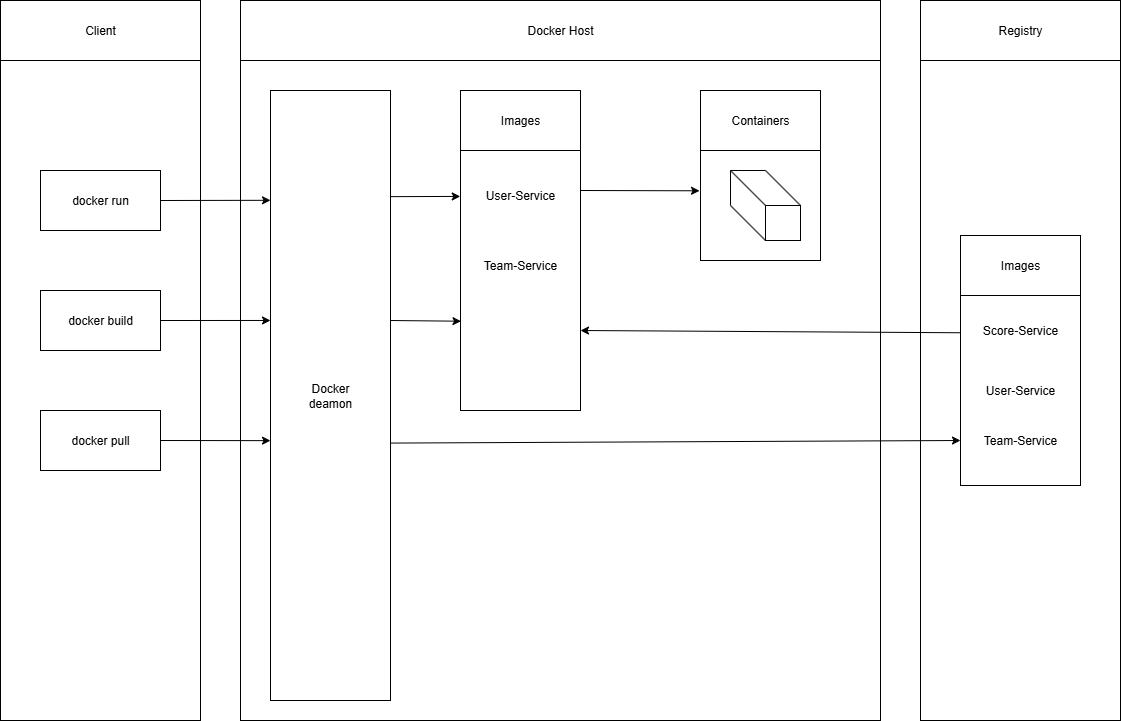
\includegraphics[width=14cm]{docker-architecture.png}
    \caption{Docker Architektur}
    \label{fig:dockerarchitektur}
\end{figure}

\subsubsection{Prinzip von Docker}
Grundlage ist das Dockerfile, eine Textdatei die Befehle beinhaltet für die Erstellung eines Docker Images. Jeder Befehl beinhaltet einen Schritt für das Image, wie zum Beispiel auf welchem Image das neue aufbauen soll, welche Dateien kopiert werden sollen oder welche Bibliotheken benötigt werden \cite{what_is_a_dockerfile_spacelift}. Dabei fügt jeder Befehl eine weitere read-only Schicht hinzu, um die Erstellungsgeschwindigkeit sowie den Speicherbedarf zu optimieren \cite{geeksforgeeks_dockerfile}.
Ein Container ist das laufende Image, wobei Abhängigkeiten und Programmcode verpackt in einer isolierten Umgebung laufen. Dies ermöglicht die Ausführbarkeit auf unterschiedlichen Geräten \cite{geeksforgeeks_what_is_docker}.
Im Gegensatz zu virtuellen Maschinen sind Docker-Container leichtgewichtig, da diese sich das Betriebsystem mit dem Host teilen und nicht wie bei virtuellen Maschinen ein eigenes benötigen. Dadurch können Container schnell starten und benötigen weniger Speicherplatz. \cite{geekflare_lightweight_container} 

\subsubsection{Docker Compose}
Docker Compose definiert Multi-Container-Applikationen in einer YAML Datei um sie einfach verwalten und starten zu können \cite{dev_to_docker_compose}. Zudem können noch Konfigurationsparameter angegeben werden, die somit nicht bei jedem Start mit angegeben werden müssen \cite{docker_what_is_docker_compose}. In dieser Diplomarbeit wird Docker Compose dafür verwendet, um die Zeitnehmer Applikation mit alle erforderlichen Konfigurationsparameter zu starten sowie alle Container die benötigt werden, um den Ablauf mit MQtt zu garantieren.


\subsubsection{Vorteile von Containern}
Mithilfe von Containern kann gewährleistet werden, dass die Applikation auf jedem Gerät läuft, egal ob auf einem Linux oder Windows Rechner, da alles, dass von der Applikation benötigt wird, in einem Container verpackt wird und dadurch unabhängig von der Umgebung ausgeführt werden kann \cite{advantages_of_docker_cantech}.
Zudem wird mit Containern in dieser Diplomarbeit die einfache Aufsetzung garantiert, da dafür nur die benötigten Images geladen werden müssen und mit dem Befehl \texttt{docker compose up} jede Applikation gestartet werden kann und keine weiteren Konfigurationsschritte erforderlich sind.

\newpage
% -------------------------------------------------------------------
\subsection{Microservices}
Microservice ist eine Architektur in der die Applikation in kleine Teile aufgeteilt wird, die unabhängig voneinander ausgeführt werden können, ohne eine andere Komponente zu benötigen. Dadurch läuft das gesamte System weiter, sollte eine Komponente ausfallen.
Jedem Service ist eine eigene Aufgabe zugeteilt und kann unabhängig von den anderen entwickelt, skaliert und deployt werden. Die Services kommunizieren untereinander über ein definiertes Protokoll wie HTTP oder Message Broker. \cite{geeksforgeeks_microservice}

\subsubsection{Vorteile von Microservices}

\begin{itemize}
    \item \textbf{Skalierbarkeit: } Da jede Komponente voneinander unabhängig ist, können neue Komponenten ohne bedenken eingeführt werden. Dabei müssen die Komponenten nicht auf der selben Technologie basieren und die beste Technologie kann gewählt werden. 
    \item \textbf{Fehlerisolierung: } Falls ein Fehler auftritt kann dieser schneller identifiziert und behebt werden.
    \item \textbf{Produktivität: } Teams können sich auf eine Komponente spezialisieren und werden nicht durch die Komplexität des Gesamtsystems beeinflusst. 
    \item \textbf{Deployment-Zeit: } Durch die strikte Trennung können Komponenten hinzugefügt beziehungsweise aktualisiert werden ohne Einfluss auf das Gesamtsystem \cite{atlassian_microservice}.
\end{itemize}

\subsubsection{Kubernetes}
Kubernetes ist eine Open-Source-Platform zur Verwaltung containerisierter Applikationen. Es übernimmt Skalierung und automatische Wiederherstellung bei Ausfällen.
Sollte eine Komponente ausfallen, wird er neu gestartet um ein funktionales System zu gewährleisten. Sollte auf einer Komponente eine hohe Last liegen, wird automatisch eine weitere Komponente dazugeschaltet \cite{kubernetes_overview}.

\newpage

\subsubsection{Architektur von Kubernetes}

\begin{figure}[h]
    \centering
    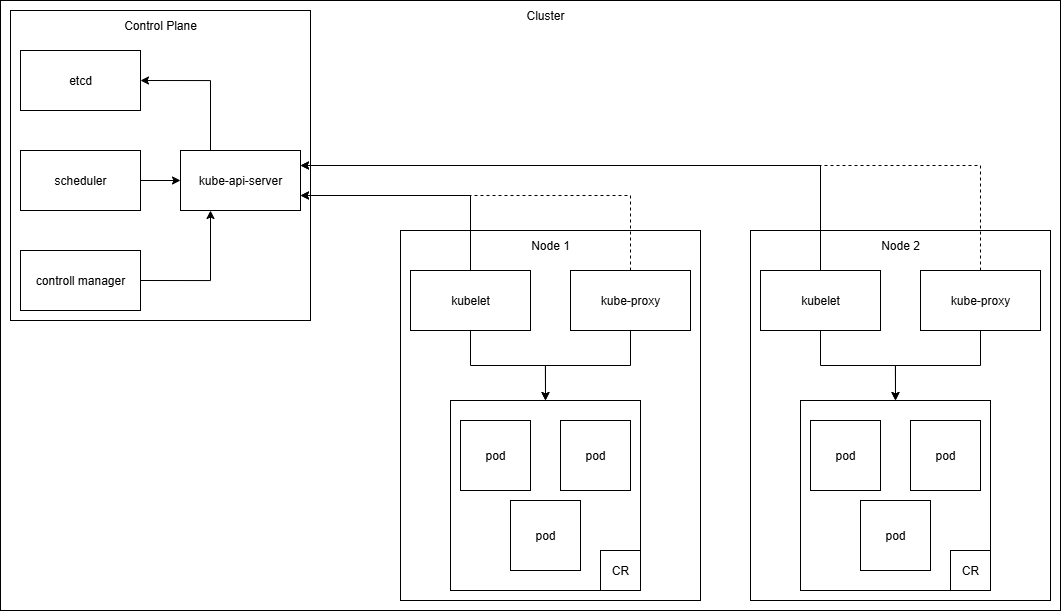
\includegraphics[width=14cm]{kubernetes_cluster_components.png}
    \caption{Kubernetes Cluster Komponenten}
    \label{fig:kubernetesclustercomponents}
\end{figure}

\begin{itemize}
    \item \textbf{Control plane: } Verwaltet den Zustand des Clusters und trifft Entscheidungen, um den gewünschten Zustand herzustellen.
    \begin{itemize}
        \item \textbf{kube-api-server: } Schnittstelle für die Kubernetes API.
        \item \textbf{etcd: } Konsistenter und hochberfügbarer Speicher für die Cluster-Daten
        \item \textbf{scheduler: } Weist neu erstellten Pods einer Node zu.
        \item \textbf{controll-manager: } Führt verschiedene Controller Prozesse aus wie etwa das abgleichen des Soll- und Ist-Zustand. Weicht dieser ab, werden Maßnahmen eingeleitet, um den Zustand wiederherzustellen
    \end{itemize}
    \item \textbf{Node: } Stellt Rechenressourcen für die Ausführung von Pods bereit.
    \begin{itemize}
        \item \textbf{kubelet: } Stellt sicher, dass ein Container in einem Pods läuft.
        \item \textbf{kube-proxy: } Verwaltet Netzwerkregeln auf Nodes, durch die Netzwerkkommunikation zu Services ermöglicht wird.
        \item \textbf{Container runtime: } Verantwortlich für die Ausführung der Container \cite{kubernetes_architektur}.
    \end{itemize}
\end{itemize}

\newpage

\subsubsection{Ressourcen von Kubernetes}

In Kubernetes werden Anwendungen über Ressourcen beschrieben, die den Soll-Zustand des Clusters definieren und von dessen Steuerungsebene kontinuierlich überwacht und durchgesetzt werden \cite{kubernetes_objects}.

\begin{itemize}
    \item \textbf{Pod: } Kleinste deploybare Einheit in Kubernetes. Enthält einen oder mehrere Container \cite{kubernetes_pods}.
    \item \textbf{Deployment: } Definiert den gewünschten Zustand der Pods und die Anzahl der auszuführenden Instanzen. \cite{kubernetes_deployment}.
    \item \textbf{Service: } Stellt eine Netzwerkadresse für Pods bereit und ermöglicht deren Erreichbarkeit innerhalb des Clusters \cite{kubernetes_service}.
    \item \textbf{Ingress: } Ermöglicht den externen Zugriff auf Services und definiert Regeln für die Weiterleitung von HTTP-Anfragen \cite{kubernetes_ingress}.
    \item \textbf{PersistentVolumeClaim: } Stellen persistenten Speicher für Pods bereit \cite{kubernetes_pvc}.
    \item \textbf{StatefulSet: } Verwaltet zustandsbehaftete Anwendungen und gewährleistet eine stabile Identität sowie eine dauerhafte Speicherung der Daten \cite{kubernetes_stateful_set}
\end{itemize}

\newpage
% -------------------------------------------------------------------
\subsection{MQTT}
% Autor: Niklas | Umfang: 1–2 Seiten
% TODO: Wie MQTT funktioniert (Publish/Subscribe)
MQTT (Message Queuing Telemetry Transport) ist ein leichtgewichtiges Nachrichten Protokoll für die Kommunikation zwischen verschiedenen Geräten. Verwendet dabei wird das Publish/Subscribe-Modell. Hierbei kommunizieren die Geräte nicht direkt untereinander, sondern senden ihre Daten an einen zentralen Broker. Ein Gerät veröffentlich eine Nachricht zu einem bestimmten Topic (Publish). Andere Geräte können dieses Topic abbonieren (Subscribe) und erhalten dadurch die Daten \cite{geeksforgeeks_mqtt}.

\begin{figure}[h]
    \centering
    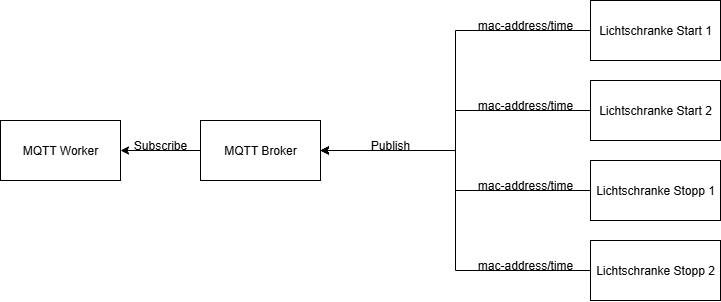
\includegraphics[width=14cm]{mqtt_pub_sub.png}
    \caption{MQTT Publish Subscribe Grafik}
    \label{fig:mqttpubsubgrafik}
\end{figure}

\newpage

\newpage

% Technologieauswahl
% ==============================================================
% Kapitel 3: Technologieauswahl
% ==============================================================

\section{Technologieauswahl}

\subsection{GitHub}
Für die Versionskontrolle des Projekts wurde GitHub ausgewählt. GitHub ist eine webbasierte Plattform zur Verwaltung und Zusammenarbeit an Softwareprojekten, die auf dem Versionsverwaltungssystem Git basiert \cite{what_is_github}. Durch die Verwendung von Git können Änderungen am Quellcode nachvollziehbar dokumentiert und verschiedene Versionen des Projekts verwaltet werden. Dadurch ist es beispielsweise möglich, Änderungen nachzuverfolgen, frühere Versionen wiederherzustellen und unabhängig voneinander an verschiedenen Entwicklungsständen zu arbeiten \cite{git_version_control} \cite{git_branching}.

Ein weiterer Grund für die Wahl von GitHub ist die umfangreiche Integration zusätzlicher Entwicklungs- und Deployment-Werkzeuge. Insbesondere ermöglicht GitHub Actions die Automatisierung von Arbeitsabläufen wie dem Ausführen von Tests, dem Erstellen von Anwendungen und dem automatisierten Deployment. Dadurch können bestimmte Schritte des Entwicklungsprozesses bei Änderungen am Quellcode automatisch ausgeführt werden \cite{github_actions}.

Zusätzlich wird die GitHub Container Registry (GHCR) verwendet. Diese ermöglicht die Speicherung und Verwaltung der im Projekt erstellten Docker-Container-Images direkt innerhalb von GitHub. Dadurch können die erstellten Images zentral verwaltet und beispielsweise für die Bereitstellung der Anwendung in einer Kubernetes-Umgebung verwendet werden \cite{github_container_registry}.

\subsection{Docker}
Zur Containerisierung wurde Docker gewählt, da dadurch die einzelnen Services plattformunabhängig bereitgestellt werden können. Die benötigten Abhängigkeiten und Laufzeitumgebungen werden dabei gemeinsam mit den Services definiert, wodurch eine einheitliche Ausführungsumgebung entsteht \cite{opc_router_docker}. Aufgrund der weiten Verbreitung und umfangreichen Dokumentation eignet sich Docker besonders für die Umsetzung und den Betrieb der Anwendung auf unterschiedlichen Systemen, beispielsweise einem Raspberry Pi oder einem Server.

\subsection{Kubernetes}
Für die Orchestrierung der Microservices wurde Kubernetes gewählt, da es eine automatisierte Verwaltung und zuverlässige Bereitstellung der einzelnen Services ermöglicht. Kubernetes übernimmt dabei unter anderem die Überwachung der Container, deren Neustart bei Fehlern sowie die Skalierung der Services. Dadurch eignet es sich besonders für eine Architektur, bei der mehrere voneinander unabhängige Microservices betrieben werden \cite{kubernetes_overview}.

Alternativ wären beispielsweise Docker Compose oder Docker Swarm möglich gewesen. Docker Compose ist jedoch hauptsächlich für die Verwaltung von Containern in kleineren und weniger komplexen Umgebungen ausgelegt und bietet im Vergleich zu Kubernetes weniger Möglichkeiten zur Skalierung und Ausfallsicherheit. Docker Swarm bietet zwar ähnliche Funktionen wie Kubernetes, verfügt jedoch über weniger umfangreiche Funktionen \cite{docker_swarm_vs_kubernetes}. Aufgrund der hohen Verbreitung, der umfangreichen Funktionalitäten und der guten Unterstützung für Microservice-Architekturen wurde daher Kubernetes als Orchestrierungsplattform ausgewählt.

\subsection{Redis}
Für die Zwischenspeicherung der zeitkritischen Zeitstempel wurde Redis gewählt, da diese nur für einen kurzen Zeitraum benötigt werden und eine schnelle Verarbeitung erforderlich ist. Durch die Speicherung im Arbeitsspeicher ermöglicht Redis sehr kurze Zugriffszeiten und eignet sich daher besonders für temporäre Daten. Zusätzlich können die gespeicherten Daten mithilfe einer Ablaufzeit (TTL) automatisch nach einem definierten Zeitraum gelöscht werden. Dadurch wird verhindert, dass nicht mehr benötigte Zeitstempel dauerhaft gespeichert werden \cite{redis_key_expiration}.

\subsection{Eclipse Mosquitto}
Für die Umsetzung des MQTT-Brokers wurde Eclipse Mosquitto gewählt, da es sich um einen leichtgewichtigen und Open-Source-MQTT-Broker handelt, der speziell für die Kommunikation über das MQTT-Protokoll entwickelt wurde. Dadurch eignet sich Mosquitto besonders für die Verarbeitung der von den Lichtschranken gesendeten Nachrichten und lässt sich zudem einfach in die bestehende Docker-Infrastruktur integrieren \cite{eclipse_mosquitto}.

\subsection{NextJs}
Für die Entwicklung der Zeitnehmer Applikation wurde Next.js gewählt, da es eine moderne und leistungsfähige Grundlage für die Entwicklung von Webanwendungen bietet. Durch die auf React basierende Architektur ermöglicht Next.js eine strukturierte Entwicklung wiederverwendbarer Komponenten. Zudem bietet das Framework Funktionen wie serverseitiges Rendering, Routing und eine optimierte Auslieferung der Anwendung. Dadurch konnte eine übersichtliche, performante und gut erweiterbare Benutzeroberfläche für das Projekt umgesetzt werden \cite{nextjs_docs}.

\subsection{shadcn/ui}
Für die Gestaltung der Benutzeroberfläche wurde shadcn/ui gewählt, da es eine Sammlung wiederverwendbarer und anpassbarer UI-Komponenten für React-Anwendungen bereitstellt. Die Komponenten lassen sich flexibel an das bestehende Design anpassen und ermöglichen dadurch eine einheitliche und übersichtliche Benutzeroberfläche. Zudem basiert shadcn/ui auf etablierten Technologien wie Tailwind CSS und Radix UI, wodurch sich die Komponenten gut in die bestehende Next.js-Anwendung integrieren lassen \cite{shadcn_ui_docs}.
\newpage

% Systemarchitektur
% ==============================================================
% Kapitel 4: Systemarchitektur
% ==============================================================

\section{Systemarchitektur}

% -------------------------------------------------------------------
\subsection{Überblick}

\begin{figure}[h]
    \centering
    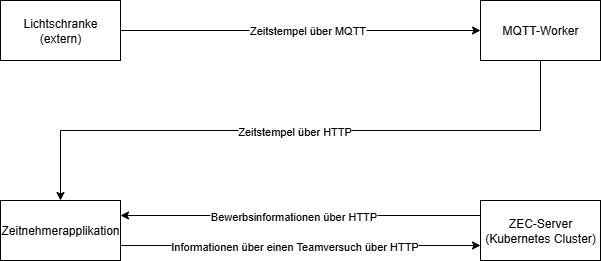
\includegraphics[width=14cm]{zec_systemarchitektur.png}
    \caption{ZEC Systemarchitektur}
    \label{fig:zec_systemarchitektur}
\end{figure}

Das Zeitmesssystem der Zero-Emission-Challenge (ZEC) besteht aus vier zentralen Komponenten: einer bereits bestehenden Lichtschranke, dem MQTT-Worker, der Zeitnehmerapplikation und dem von Diplomarbeitspartner Darnhofer David implementierten ZEC-Server. Die Lichtschranke erfasst beim Auslösen einen Zeitstempel und übermittelt diesen über das MQTT-Protokoll an den MQTT-Worker. Dieser empfängt die Zeitstempel und stellt sie über eine \gls{API} für die weiteren Komponenten des Systems bereit. Die Zeitnehmerapplikation wird von den Zeitnehmern verwendet, um die Versuche der teilnehmenden Teams zu erfassen. Der ZEC-Server nimmt die von der Zeitnehmerapplikation übermittelten Informationen entgegen und stellt zusätzlich Daten, beispielsweise zu Teams, deren Mitgliedern und Fahrern, über eine \gls{API} zur Verfügung.

\newpage

Um den Ablauf eines Versuches besser zu verstehen, wurde dieser im folgenden Sequenzdiagramm abgebildet:

\begin{figure}[h]
    \centering
    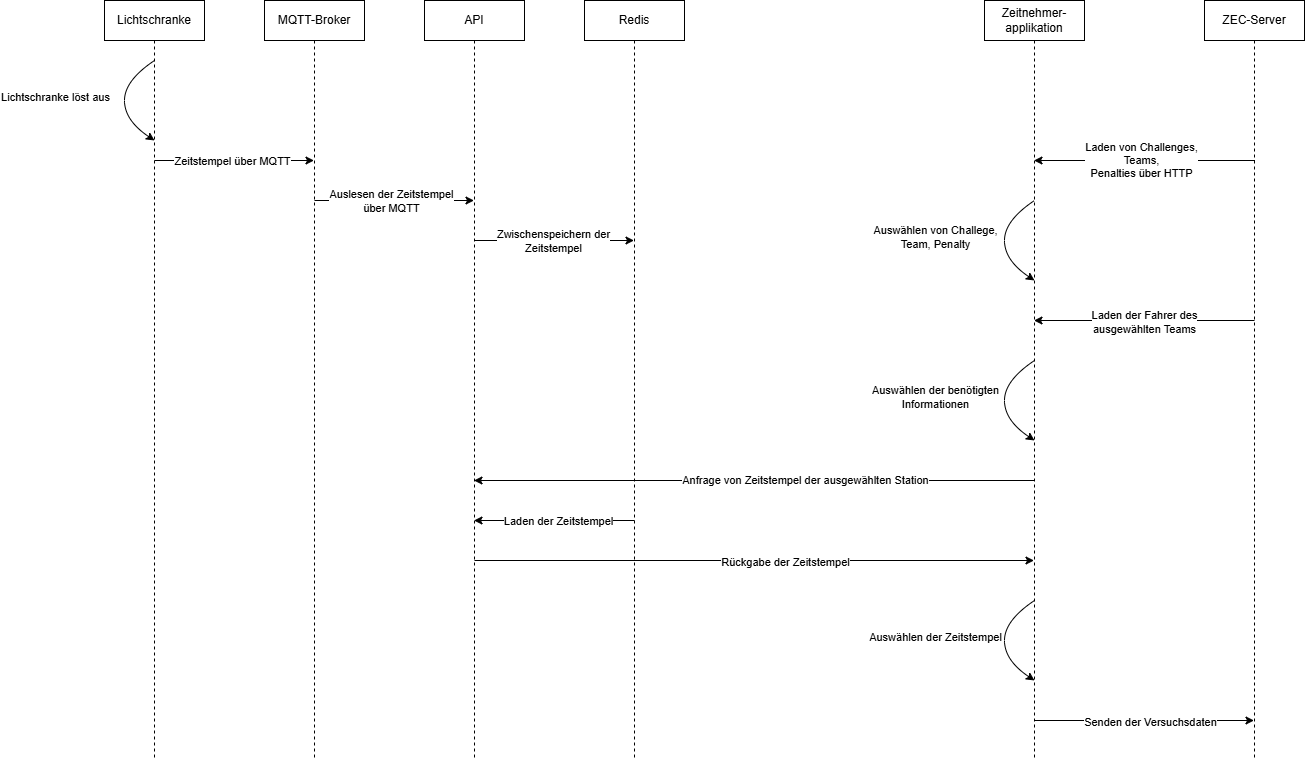
\includegraphics[width=14cm]{sequenzdiagram_zec.png}
    \caption{Sequenzdiagramm Ablauf}
    \label{fig:sequenzdiagram_ablauf}
\end{figure}

Hierbei ist zu beachten, dass der \textbf{MQTT-Worker} im Sequenzdiagramm in seine drei wesentlichen Komponenten MQTT-Broker, \gls{API} und Redis aufgeteilt dargestellt wird.

Jedes Mal, wenn ein Fahrer eine Lichtschranke passiert und dadurch ein Versuch gestartet oder beendet wird, übermittelt die Lichtschranke den dabei erfassten Zeitstempel über das MQTT-Protokoll an den MQTT-Broker. Die Zeitstempel werden anschließend von der \gls{API} des \textit{MQTT-Workers} ausgelesen und für einen bestimmten Zeitraum in Redis zwischengespeichert.

Beim Start der Zeitnehmerapplikation werden zunächst alle verfügbaren Challenges, Teams und Penalties vom \textit{ZEC-Server} geladen. Nachdem der Zeitnehmer die benötigten Einstellungen vorgenommen und die gewünschten Daten ausgewählt hat, werden zusätzlich die Fahrer des ausgewählten Teams vom \textit{ZEC-Server} geladen.

Sofern das \textit{Activate}-Feld in der Zeitnehmerapplikation aktiviert wurde, werden während des weiteren Ablaufs fortlaufend die Zeitstempel der zur ausgewählten Station gehörenden Lichtschranken beim MQTT-Worker angefragt. Die vom MQTT-Worker zurückgegebenen Zeitstempel können anschließend vom Zeitnehmer ausgewählt und für die Zeitmessung des Versuches verwendet werden.

Nachdem der Zeitnehmer das Formular vollständig ausgefüllt und die benötigten Zeitstempel ausgewählt hat, werden die daraus ermittelten Versuchsdaten an den \textit{ZEC-Server} übermittelt.

\newpage

\subsubsection{MQTT-Worker}

\begin{figure}[h]
    \centering
    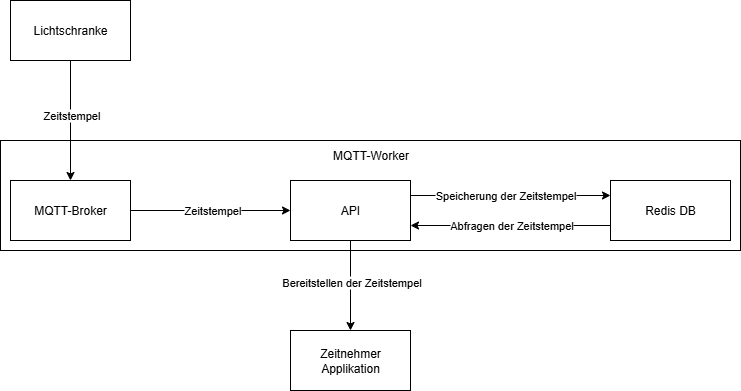
\includegraphics[width=14cm]{mqtt_worker_architektur.png}
    \caption{MQTT-Worker Architektur}
    \label{fig:mqtt_worker_architektur}
\end{figure}

Der MQTT-Worker besteht aus einem MQTT-Broker und einer \gls{API}. Der MQTT-Broker empfängt die von der Lichtschranke über das MQTT-Protokoll übertragenen Zeitstempel. Diese werden von der \gls{API} automatisch verarbeitet und in der Redis-Datenbank (\gls{DB}) zwischengespeichert. Wird ein Zeitstempel über die \gls{API} abgefragt, werden die entsprechenden Daten aus der Redis-Datenbank geladen und dem anfragenden System zur Verfügung gestellt.

Folgende \gls{API}-Endpunkte werden vom \textit{MQTT-Worker} zur Verfügung gestellt:

\texttt{/timestamps/<mac-adresse>}

Der Endpunkt ermöglicht das Abrufen der für die angegebene MAC-Adresse gespeicherten Zeitstempel. Das Response-Modell ist dabei wie folgt aufgebaut:

\begin{lstlisting}
{
    "timestamp": [
        "Timestamp_1",
        "Timestamp_2",
        "Timestamp_..."
    ]
}
\end{lstlisting}

\newpage

\subsection{Zeitnehmerapplikation}

Die Zeitnehmerapplikation wurde mit Next.js \cite{nextjs_docs} umgesetzt und ist für das Erstellen und Verwalten der Versuche verantwortlich. Sie wird von den Zeitnehmern verwendet und lädt die für die Zeitmessung benötigten Informationen, wie beispielsweise Challenges, Teams und deren zugehörige Fahrer. Jeder Challenge sind vier Lichtschranken mit jeweils einer eindeutigen MAC-Adresse zugeordnet. Sobald das Pairing aktiviert wurde, werden anhand dieser MAC-Adressen die zugehörigen Zeitstempel beim MQTT-Worker abgefragt. Der ZEC-Server erfordert für den Zugriff normalerweise eine Authentifizierung. Da für die Zeitnehmerapplikation jedoch keine Benutzeranmeldung vorgesehen ist, wird stattdessen ein API-Key zur Authentifizierung der Anfragen verwendet. Nach Abschluss eines Versuchs werden die erfassten Daten an den ZEC-Server übermittelt, wo sie zur weiteren Verarbeitung und Auswertung verwendet werden.


\begin{figure}[h]
    \centering
    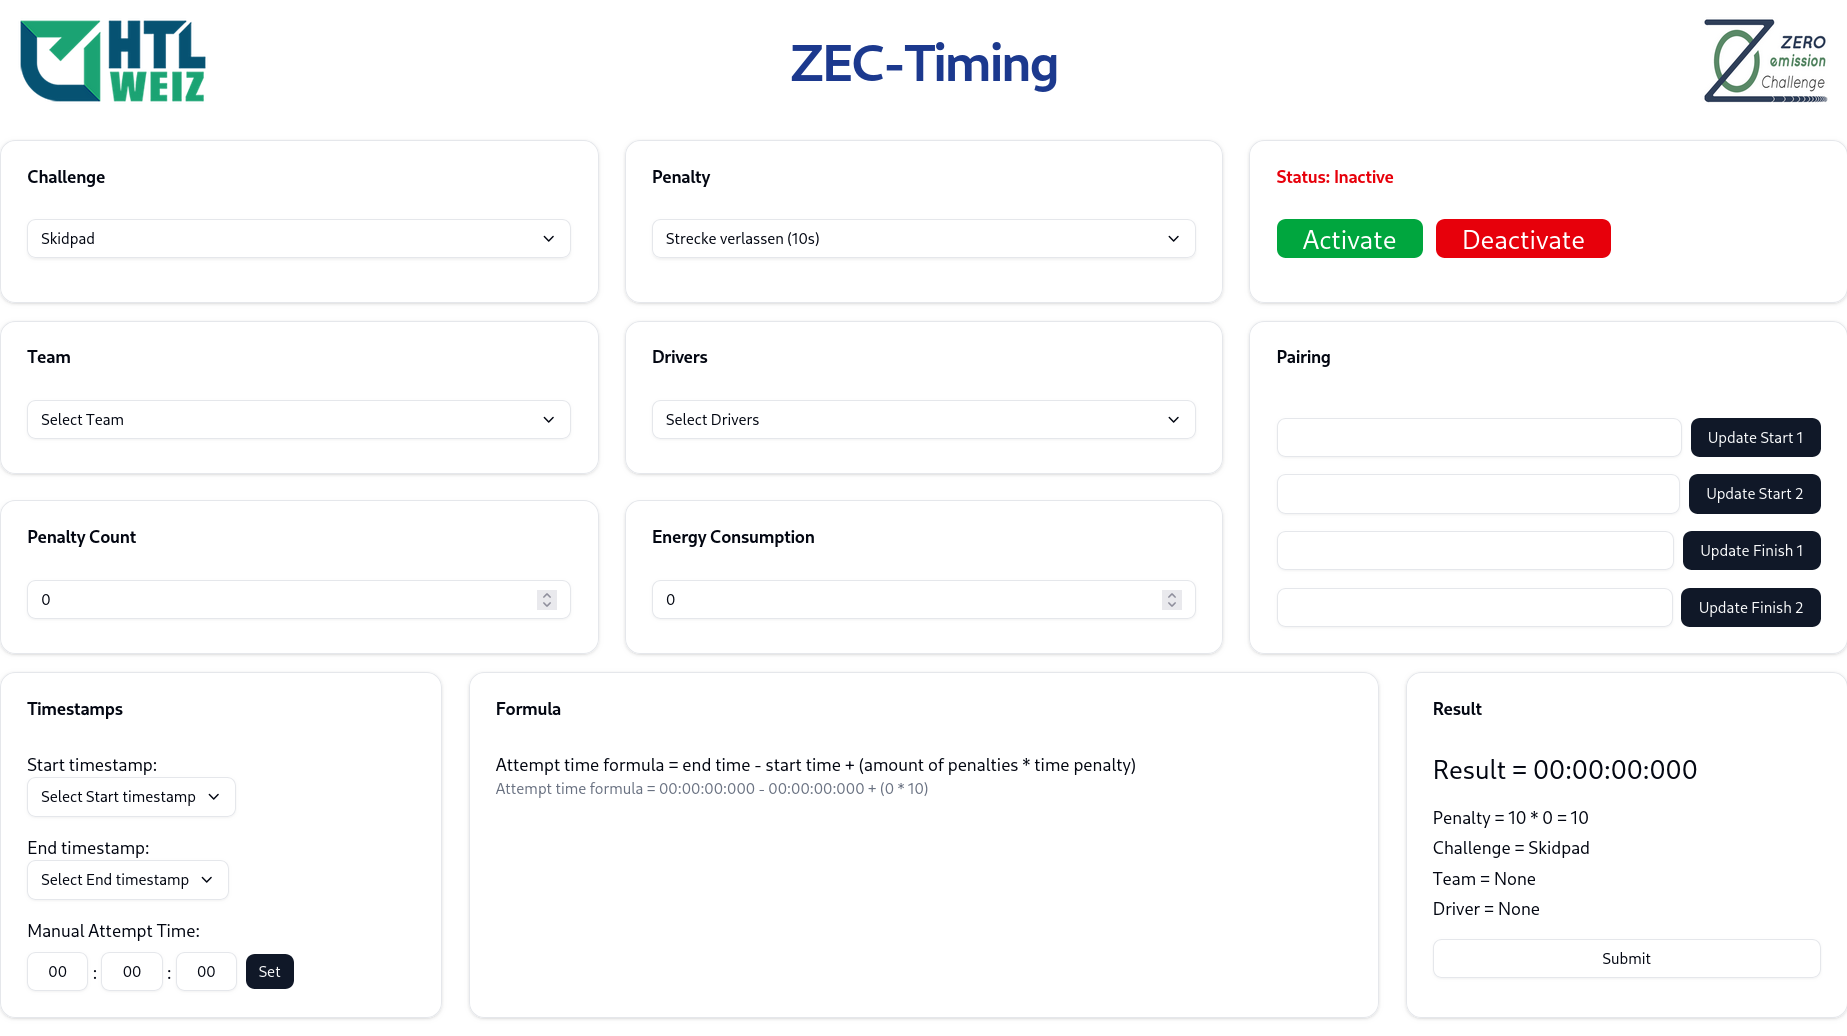
\includegraphics[width=14cm]{zeitnehmerapplikation.png}
    \caption{Zeitnehmerapplikation}
    \label{fig:zeitnehmerapplikation}
\end{figure}

\subsection{ZEC-Server}

Die Orchestrierung des von Diplomarbeitspartner Darnhofer David implementierten ZEC-Servers wurde mittels Kubernetes realisiert. Die dafür erforderliche Implementierung wurde vom Diplomarbeitspartner David Darnhofer durchgeführt.

\newpage

% Implementation
% ==============================================================
% Kapitel 05: Implementation
% ==============================================================

\section{Implementation}

\subsection{Github Actions}

Nach jeder Änderung am Quellcode der auf GitHub gepusht wird, wird automatisch ein GitHub-Actions-Workflow ausgelöst, der die Anwendung erstellt und als Docker-Image verpackt \cite{github_actions}. Dieses Image wird anschließend in der GitHub Container Registry veröffentlicht und steht dort für das Deployment zur Verfügung \cite{github_container_registry}. Dadurch wird beim Deployment lediglich das bereits fertig erstellte Image benötigt und nicht mehr der Quellcode selbst. Zusätzlich verkürzt sich die Deployment-Zeit, da der aufwendige Build-Prozess bereits im Rahmen des GitHub-Actions-Workflows durchgeführt wird und auf dem Zielsystem nicht erneut ausgeführt werden muss.
Hier ein Beispielscode, bei dem die Zeitnehmerapplikation gebaut wird:

\begin{CodeBox}
name: Desktop App CI Job
on:
  push:
    branches: ["<Auf welchen Branch er hoert>"]
jobs:
  build-desktop-app:
    runs-on: ubuntu-latest
    steps:
      - uses: actions/checkout@v3
      - name: Login
        uses: docker/login-action@v3
        with:
          registry: ghcr.io
          username: ${{ github.repository_owner }}
          password: ${{ secrets.GITHUB_TOKEN }}
      - name: Build desktop app
        uses: docker/build-push-action@v6
        with:
          platforms: linux/amd64
          push: true
          tags: <Name des Docker-Images>
          context: <Verzeichnis der Anwendung>
\end{CodeBox}

Der Workflow wird durch einen Push auf den definierten Branch ausgelöst. Zunächst wird mit der Aktion \texttt{actions/checkout} der aktuelle Quellcode des Projekts aus dem Repository geladen. Anschließend erfolgt die Anmeldung an der GitHub Container Registry, damit das erstellte Docker-Image dort veröffentlicht werden kann. Für die Anmeldung wird das von GitHub Actions bereitgestellte \texttt{GITHUB\_TOKEN} verwendet. Im letzten Schritt wird mit der \texttt{docker/build-push-action} das Docker-Image aus dem angegebenen Verzeichnis erstellt und anschließend in die Container Registry hochgeladen. Durch die Angabe der Plattform \texttt{linux/amd64} wird sichergestellt, dass das Image für die Zielumgebung geeignet ist \cite{docker_build_push_action}.

Dieser Prozess ermöglicht es, den Build der Anwendung vollständig zu automatisieren. Änderungen am Quellcode werden dadurch direkt in ein aktualisiertes Docker-Image überführt, welches anschließend für das Deployment verwendet werden kann. Dadurch wird der Build-Prozess von der eigentlichen Deployment-Umgebung getrennt.

\subsection{MQTT-Worker}

\subsubsection{MQTT-Broker}

Der MQTT-Broker wird als eigener Docker-Container auf Basis des offiziellen Eclipse-Mosquitto-Images betrieben. Über das Dockerfile werden zusätzlich benötigte Dateien in den Container kopiert und ein eigenes Entrypoint-Skript als Startpunkt definiert. Dadurch kann die Konfiguration des Brokers beim Start des Containers automatisiert vorbereitet werden.

\begin{CodeBox}
FROM eclipse-mosquitto:latest

RUN apk add --no-cache bash

COPY docker-entrypoint.sh /docker-entrypoint.sh
RUN chmod +x /docker-entrypoint.sh

COPY mosquitto.conf /mosquitto/config/mosquitto.conf

ENTRYPOINT ["/docker-entrypoint.sh"]
CMD ["/usr/sbin/mosquitto", "-c", "/mosquitto/config/mosquitto.conf"]
\end{CodeBox}

Das Entrypoint-Skript legt anhand der über Umgebungsvariablen bereitgestellten Zugangsdaten einen MQTT-Benutzer an. Werden keine Zugangsdaten angegeben, werden Standardwerte verwendet. Die erzeugte Passwortdatei wird anschließend mit den notwendigen Dateiberechtigungen versehen, bevor der MQTT-Broker gestartet wird.

\begin{CodeBox}
\#\!/bin/bash
set -e

MQTT_USER="${MQTT_USER:-admin}"
MQTT_PASSWORD="${MQTT_PASSWORD:-password}"

echo "Creating MQTT user: $MQTT_USER"

mosquitto_passwd -c -b /mosquitto/config/passwd "$MQTT_USER" "$MQTT_PASSWORD"
chown mosquitto:mosquitto /mosquitto/config/passwd
chmod 600 /mosquitto/config/passwd

exec "$@" 
\end{CodeBox}

Die eigentliche Konfiguration des Brokers erfolgt über die Datei \texttt{mosquitto.conf}. Der Broker lauscht auf Port 1883 und erlaubt keine anonymen Verbindungen. Stattdessen müssen sich Clients mit den in der Passwortdatei hinterlegten Zugangsdaten authentifizieren. Zudem werden die Log-Ausgaben nicht dauerhaft in einer Datei gespeichert, sondern an die Standardausgabe des Containers weitergeleitet. Dadurch werden unnötige Schreibvorgänge auf der SD-Karte vermieden und deren Verschleiß reduziert.

\begin{CodeBox}
listener 1883
allow_anonymous false
password_file /mosquitto/config/passwd
log_dest stdout
\end{CodeBox}

\newpage

\subsubsection{API}

Beim Empfang einer MQTT-Nachricht wird zunächst die übermittelte JSON-Nachricht verarbeitet und die darin enthaltene MAC-Adresse sowie der Zeitstempel ausgelesen. Da die MAC-Adresse im Feld \texttt{esp\_id} zusammen mit dem Präfix \texttt{ESP32-} übertragen wird, wird dieses Präfix vor der weiteren Verarbeitung entfernt. Anschließend wird der Zeitstempel anhand der MAC-Adresse in Redis gespeichert. Ein entsprechendes Codebeispiel ist im Anhang zu finden.

Für die Speicherung wird pro Lichtschranke ein eigener Redis-Key nach dem Schema \texttt{timestamps:{mac}} verwendet. Da die Zeitstempel nur für einen begrenzten Zeitraum benötigt werden und nach ihrer Verarbeitung nicht dauerhaft gespeichert werden müssen, wird für jeden Zeitstempel ein Ablaufzeitpunkt festgelegt. Dieser wird aus der aktuellen Zeit und dem in \texttt{TIMESTAMP\_EXPIRE\_TIME} festgelegten Zeitraum berechnet. Nach Ablauf dieses Zeitraums wird der Zeitstempel aus der Zwischenspeicherung entfernt und steht nicht mehr zur Verfügung.

Der Wert von \texttt{TIMESTAMP\_EXPIRE\_TIME} wird über die Konfiguration des Containers festgelegt und muss beim Start des Containers als Umgebungsvariable angegeben werden. Dadurch kann die Speicherdauer der Zeitstempel flexibel angepasst werden, ohne Änderungen am Quellcode vornehmen zu müssen.
Die Umsetzung dieser Funktion ist im folgenden Code umgesetzt:

\begin{CodeBox}
def add_timestamp(mac: str, timestamp: str):
    key = f"timestamps:{mac}"
    expires_at = time.time() + settings.TIMESTAMP_EXPIRE_TIME

    redis_connection.zadd(
        key,
        {timestamp: expires_at}
    )
\end{CodeBox}

Für den Abruf der gespeicherten Zeitstempel stellt der MQTT-Worker einen \gls{API}-Endpunkt unter bereit, der über die MAC-Adresse der jeweiligen Lichtschranke aufgerufen wird. Da die MAC-Adresse bei der Anfrage mit Bindestrichen übergeben werden muss, werden diese zunächst durch Doppelpunkte ersetzt, um das Format des zugehörigen Redis-Keys herzustellen. Anschließend werden die gespeicherten Zeitstempel aus Redis abgefragt.

Vor der Rückgabe werden zunächst alle Zeitstempel entfernt, deren Ablaufzeitpunkt bereits erreicht wurde. Hierfür werden die aktuell abgelaufenen Einträge aus der Redis Sorted Set entfernt. Befinden sich danach keine gültigen Zeitstempel mehr unter dem entsprechenden Key, wird eine HTTP-404-Fehlermeldung zurückgegeben. Andernfalls werden die noch gültigen Zeitstempel aus Redis geladen und über die API an die anfragende Anwendung zurückgegeben. Die Umsetzung des API-Endpunkts sowie die Bereinigung der abgelaufenen Zeitstempel sind im Anhang zu finden.

\newpage

\subsection{Zeitnehmerapplikation}

Um die Bedienung der Zeitnehmerapplikation zu erleichtern, wurden Auswahlmöglichkeiten, die im selben Arbeitsschritt getroffen werden, zu Gruppen zusammengefasst. Dadurch wird außerdem eine intuitive Bedienung von oben nach unten ermöglicht. Die einzelnen Auswahlmöglichkeiten sind entsprechend dem Ablauf eines Versuchs angeordnet, sodass die Anwendung schrittweise von oben nach unten abgearbeitet werden kann. Der Aufbau und die Anordnung der einzelnen Elemente können im nachfolgenden Wireframe-Diagramm nachvollzogen werden:

\begin{figure}[h]
    \centering
    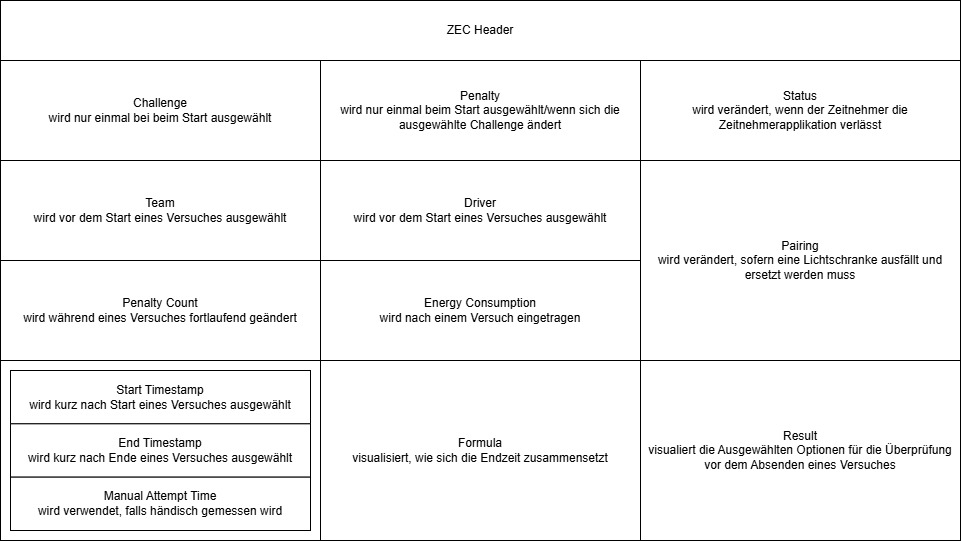
\includegraphics[width=14cm]{wireframe-zeitnehmerapplikation-erklaerung.png}
    \caption{Wireframe Zeitnehmerapplikation mit Erklärung}
    \label{fig:wireframe_zeitnehmerapplikation_erklaerung}
\end{figure}

Dabei basiert die Zeitnehmerapplikation auf wiederverwendbaren Komponenten, wodurch das Layout der Zeitnehmerapplikation schnell angepasst werden kann, ohne die grundlegende Funktionsweise der Anwendung zu beeinflussen. Die Wiederverwendbarkeit der Komponenten verkürzt zudem die Entwicklungszeit und reduziert die Fehleranfälligkeit, da bereits implementierte und getestete Komponenten mehrfach verwendet werden können.

\newpage

\subsubsection{Kommunikation mit ZEC-Server}

Die Zeitnehmerapplikation benötigt für ihre Verwendung verschiedene Daten vom ZEC-Server. Die dafür bereitgestellten Endpunkte sind durch eine Authentifizierung geschützt. Da für die Zeitnehmerapplikation keine Anmeldung mittels Benutzername und Passwort vorgesehen ist, wird für Anfragen, die eine Authentifizierung erfordern, stattdessen ein API-Key verwendet. Dieser wird beim Start des Containers als Umgebungsvariable hinterlegt und von der Anwendung für die Authentifizierung der Anfragen verwendet.

Ein entsprechendes Codebeispiel ist im Anhang zu finden.

\subsubsection{Kommunikation mit MQTT-Worker}

Durch den Einsatz des MQTT-Workers muss die Zeitnehmerapplikation nicht direkt über das MQTT-Protokoll mit den Lichtschranken kommunizieren. Stattdessen stellt der MQTT-Worker die empfangenen Zeitstempel über eine HTTP-\gls{API} bereit. Dadurch kann die Zeitnehmerapplikation, analog zur Kommunikation mit dem ZEC-Server, HTTP für die Kommunikation verwenden.

Dadurch wird für die Kommunikation der Zeitnehmerapplikation mit den angebundenen Diensten ein einheitliches Protokoll verwendet. Dies vereinfacht die Implementierung, da die Anwendung lediglich HTTP-Anfragen verarbeiten muss und keine zusätzliche MQTT-Kommunikation benötigt.

Ein entsprechendes Codebeispiel ist im Anhang zu finden.

\newpage

\subsection{Kubernetes Cluster}

Wie bereits in 5.2.4 beschrieben, werden Kubernetes Anwendung über Ressourcen beschrieben

\subsubsection{Deployment}

Ein Deployment beschreibt in Kubernetes, wie eine Anwendung innerhalb des Clusters bereitgestellt und verwaltet werden soll. Dabei wird unter anderem festgelegt, welches Container-Image verwendet wird, wie viele Instanzen der Anwendung ausgeführt werden und welche Ressourcen dafür zur Verfügung stehen.

Das folgende Beispiel zeigt die grundlegende Struktur eines Deployments:

\begin{CodeBox}
apiVersion: apps/v1
kind: Deployment
metadata:
  name: <name>-deployment
  labels:
    app: <name>
spec:
  replicas: <Anzahl der Pod-Instanzen>
  selector:
    matchLabels:
      app: <name>
  template:
    metadata:
      labels:
        app: <name>
    spec:
      containers:
        - name: <name>
          image: <Zu verwendendes Container-Image>
          ports:
            - containerPort: <Port, auf dem die Anwendung im Container erreichbar ist>
          env:
            - name: <Name der Umgebungsvariable>
              value: <Wert der Umgebungsvariable>
          resources:
            requests:
              cpu: <Minimal benoetigte CPU-Ressourcen>
              memory: <Minimal benoetigter Arbeitsspeicher>
            limits:
              cpu: <Maximal verwendbare CPU-Ressourcen>
              memory: <Maximal verwendbarer Arbeitsspeicher>
\end{CodeBox}

Über \texttt{replicas} wird die gewünschte Anzahl an Pod-Instanzen festgelegt. Der \texttt{selector} definiert anhand von Labels, welche Pods zu dem Deployment gehören. Im \texttt{template} wird anschließend die Konfiguration der zu erstellenden Pods beschrieben. Dazu gehören unter anderem der Name des Containers, das zu verwendende Container-Image und der Port, auf dem die Anwendung innerhalb des Containers erreichbar ist.

Über den Abschnitt \texttt{env} können Umgebungsvariablen an den Container übergeben werden. Diese werden beispielsweise für die Konfiguration der Anwendung oder für die Verbindung zu anderen Services verwendet \cite{kubernetes_deployment_deployment}. Mit \texttt{resources} werden zusätzlich Ressourcenanforderungen und -begrenzungen definiert. Die \texttt{requests} geben an, welche Ressourcen für den Container mindestens benötigt werden, während die \texttt{limits} die maximal verwendbaren CPU- und Arbeitsspeicherressourcen festlegen \cite{kubernetes_deployment_ressource}.

\newpage

\subsubsection{Service}

Ein Kubernetes-Service stellt eine feste Zugriffsmöglichkeit auf die Pods einer Anwendung innerhalb des Clusters bereit. Über den \texttt{selector} wird anhand des Labels festgelegt, an welche Pods eingehende Anfragen weitergeleitet werden. Dadurch können andere Services innerhalb des Clusters über den Namen des Kubernetes-Services auf die Anwendung zugreifen, ohne die IP-Adresse eines einzelnen Pods kennen zu müssen.

Über \texttt{port} wird festgelegt, auf welchem Port der Service erreichbar ist, während \texttt{targetPort} den Port des Containers angibt, an den die Anfragen weitergeleitet werden. Im folgenden Beispiel wird der Service als interner \texttt{ClusterIP}-Service betrieben. Dadurch ist der zugehörige Pod nicht direkt von außerhalb des Kubernetes-Clusters erreichbar. Der Zugriff auf den Service ist somit auf andere Komponenten innerhalb des Clusters beschränkt:

\begin{CodeBox}
apiVersion: v1
kind: Service
metadata:
  name: <name>-service
spec:
  selector:
    app: <name>
  ports:
   - protocol: TCP
     port: <Port des Services>
     targetPort: <Port des Containers>
\end{CodeBox}

Da kein anderer Service-Typ wie \texttt{NodePort} oder \texttt{LoadBalancer} angegeben wird, verwendet Kubernetes standardmäßig \texttt{ClusterIP}. Dadurch bleibt der Service innerhalb des Clusters erreichbar und wird nicht direkt nach außen veröffentlicht \cite{kubernetes_service}.

\newpage

\subsubsection{Persistance Volume Claim}

Ein PersistentVolumeClaim (PVC) wird in Kubernetes verwendet, um dauerhaften Speicher für einen Pod anzufordern. Dadurch können Daten unabhängig vom Lebenszyklus eines Pods gespeichert werden und bleiben beispielsweise auch nach einem Neustart oder einer Neuerstellung des Pods erhalten.

\begin{CodeBox}
apiVersion: v1
kind: PersistentVolumeClaim
metadata:
  name: <Name der Datenbank>
spec:
  accessModes:
    - ReadWriteOnce
  resources:
    requests:
      storage: <Wie viel Speicher zur Verfuegung gestellt wird>
\end{CodeBox}

Über \texttt{accessModes} wird festgelegt, wie auf den Speicher zugegriffen werden darf. Im vorliegenden System wird \texttt{ReadWriteOnce} verwendet, da jede Datenbank über einen eigenen persistenten Speicher verfügt und jeweils nur von einer Datenbankinstanz darauf zugegriffen wird. Auch wenn ein Microservice durch mehrere Pod-Instanzen skaliert wird, greifen diese nicht direkt auf das Datenbank-Volume zu, sondern kommunizieren über den zugehörigen Kubernetes-Service mit der Datenbank.

Unter \texttt{resources.requests.storage} wird die benötigte Speicherkapazität angegeben. Kubernetes versucht daraufhin, ein passendes Persistent Volume (PV) für diese Anforderung bereitzustellen \cite{kubernetes_pvc}.

\newpage

\subsubsection{Stateful Set}

Ein StatefulSet wird in Kubernetes für Anwendungen verwendet, die einen dauerhaften Zustand und eine feste Identität benötigen. In dieser Diplomarbeit wird es für die PostgreSQL-Datenbank eingesetzt.

\begin{CodeBox}
apiVersion: apps/v1
kind: StatefulSet
metadata:
  name: <name>-db
spec:
  serviceName: "<name>-db"
  replicas: <Anzahl der Datenbank-Instanzen>
  selector:
    matchLabels:
      app: <name>-db
  template:
    metadata:
      labels:
        app: <name>-db
    spec:
      containers:
        - name: postgres
          image: <Zu verwendendes Container-Image>
          ports:
            - containerPort: 5432
          env:
            - name: POSTGRES_USER
              value: <Datenbank-Benutzer>
            - name: POSTGRES_PASSWORD
              value: <Datenbank-Passwort>
            - name: POSTGRES_DB
              value: <Datenbankname>
          volumeMounts:
            - name: <Name des Speichers>
              mountPath: /var/lib/postgresql/data
          resources:
            requests:
              cpu: <Minimal benoetigte CPU-Ressourcen>
              memory: <Minimal benoetigter Arbeitsspeicher>
            limits:
              cpu: <Maximal verwendbare CPU-Ressourcen>
              memory: <Maximal verwendbarer Arbeitsspeicher>
      volumes:
        - name: <Name des Speichers>
          persistentVolumeClaim:
            claimName: <Name des PersistentVolumeClaims>
\end{CodeBox}

Das StatefulSet erstellt eine PostgreSQL-Instanz und stellt über die Umgebungsvariablen deren Benutzer, Passwort und Datenbank fest. Über \texttt{volumeMounts} wird der zuvor definierte persistente Speicher in den Container eingebunden. Dadurch bleiben die Daten auch bei einer Neuerstellung des Pods erhalten.

Durch \texttt{resources} werden außerdem die minimal benötigten und maximal verwendbaren CPU- und Speicherressourcen festgelegt \cite{kubernetes_stateful_set}.

\newpage

\subsubsection{Ingress}

Ein Ingress definiert Regeln für eingehende HTTP-Anfragen und stellt den externen Einstiegspunkt in das Kubernetes-Cluster dar. In dieser Diplomarbeit wird der Ingress ausschließlich zur Weiterleitung der Anfragen an das von Diplomarbeitspartner Darnhofer David implementierte API-Gateway verwendet. Die Weiterleitung an die einzelnen Microservices erfolgt anschließend durch das API-Gateway.

\begin{CodeBox}
apiVersion: networking.k8s.io/v1
kind: Ingress
metadata:
  name: <Name des Ingress>
  annotations:
    traefik.ingress.kubernetes.io/router.entrypoints: <Verwendeter Traefik-Einstiegspunkt>
    traefik.ingress.kubernetes.io/service.passhostheader: "<Weitergabe des Host-Headers>"
spec:
  rules:
    - host: <Verwendeter Hostname>
      http:
        paths:
          - path: <Weiterleitungspfad>
            pathType: Prefix
            backend:
              service:
                name: <Name des API-Gateway-Services>
                port:
                  number: <Port des API-Gateways>
\end{CodeBox}

Über \textbf{host} und \textbf{path} wird festgelegt, für welche eingehenden Anfragen die Weiterleitungsregel gilt. In diesem Fall werden alle Anfragen an den angegebenen Host und Pfad an den Kubernetes-Service des API-Gateways weitergeleitet. Der Ingress selbst übernimmt somit keine direkte Kommunikation mit den einzelnen Microservices.

Durch die Verwendung von Traefik als Ingress-Controller wird der eingehende HTTP-Verkehr entgegengenommen und entsprechend der definierten Regeln an das API-Gateway weitergeleitet. Dadurch bildet der Ingress eine klare Trennung zwischen dem externen Zugriff auf das System und der internen Kommunikation zwischen API-Gateway und Microservices.

\newpage

% Testen
% ==============================================================
% Kapitel 6: Testen
% ==============================================================

\section{Testen}

Da eine vollständige Automatisierung der Tests für das Gesamtsystem nur mit erheblichem Aufwand möglich ist, wurde der Ablauf eines Versuchs manuell simuliert. Hierzu wurde ein Skript ausgeführt, das einen Zeitstempel an den MQTT-Broker übermittelte. Anschließend wurden in der Zeitnehmerapplikation die Teams und deren Fahrer erfolgreich von der im Kubernetes-Cluster betriebenen ZEC-API abgerufen. Nach dem Absenden des simulierten Versuchs wurde dieser erfolgreich verarbeitet und anschließend im Leaderboard der ebenfalls im Kubernetes-Cluster betriebenen Web-Applikation angezeigt.

\section{Deployment}

\subsection{Zeitnehmerapplikation}

Die Zeitnehmerapplikation wird idealerweise auf demselben Gerät deployt, auf dem sie von den Zeitnehmern bedient wird. Hierfür kann die im Repository (unter dem Branch ZEC-Server) enthaltene \textbf{Docker-Compose-Datei} verwendet werden. Diese lädt das fertige Image aus der GitHub Container Registry und startet den Container mit den benötigten Umgebungsvariablen. Alternativ kann die Anwendung auch mit folgendem Befehl gestartet werden:

\begin{CodeBox}
docker run -d \
  --name zec-desktop-app-frontend \
  --restart unless-stopped \
  -p 5173:3000 \
  -e NEXT_PUBLIC_DESKTOP_APP_API_URL="<Adresse der ZEC-API>" \
  -e NEXT_PUBLIC_MQTT_WORKER_API_URL="<Adresse des MQTT-Workers>" \
  -e NEXT_PUBLIC_API_KEY="<API-Key>" \
  ghcr.io/niklas-maderbacher/zec-timing:desktop-app
\end{CodeBox}

Nach dem Deployment ist die Zeitnehmerapplikation unter \textbf{localhost:5173} erreichbar.

\subsection{MQTT-Worker}

Die Multicontainer-Applikation MQTT-Worker wird idealerweise auf demselben Gerät bereitgestellt, auf dem auch die ZEC-API betrieben wird. Hierfür wird die im Repository im Branch \textit{ZEC-Server} enthaltene \textbf{Docker-Compose-Datei} empfohlen, da dadurch die einzelnen Container automatisiert gestartet und konfiguriert werden und kein komplexer \textbf{docker run}-Befehl manuell ausgeführt werden muss.

\subsubsection{ZEC-Server mittels Kubernetes}

Um die vom Diplomarbeitspartner Darnhofer David entwickelte ZEC-API und Web-App mittels Kubernetes zu deployen, werden die im Repository im Branch \textit{ZEC-Server} im Verzeichnis \textit{server-cluster} enthaltenen Dateien benötigt. Darunter befindet sich auch das Skript \textit{start-stop.sh}, mit dem der Kubernetes-Cluster einfach gestartet werden kann.

Für die von Darnhofer David beschriebenen Schritte zur Konfiguration von Keycloak muss der entsprechende Microservice von außen erreichbar sein. Hierfür muss folgender Befehl ausgeführt werden:

\begin{CodeBox}
kubectl port-forward deployment/keycloak-deployment 8080:8080
\end{CodeBox}

Dadurch ist Keycloak von außen erreichbar und kann entsprechend der von Darnhofer David beschriebenen Vorgehensweise konfiguriert werden. Dazu zählen unter anderem das Hinzufügen des Realms sowie das Ändern der Admin- und Login-Zugangsdaten. Anschließend müssen die geänderten Zugangsdaten im Deployment in der Datei \textit{deployment.yaml} eingetragen und mit folgendem Befehl angewendet werden:

\begin{CodeBox}
kubectl apply -f deployment.yaml
\end{CodeBox}

Nach dem Anwenden der Konfiguration muss einige Zeit gewartet werden, bis alle Services gestartet und betriebsbereit sind. Anschließend ist die \textit{ZEC-API} unter \textit{zec.local} und die \textit{Web-App} unter \textit{zec-timing.local} erreichbar.

Sollen diese Adressen geändert werden, müssen die entsprechenden Einträge in der Datei \textit{ingress.yaml} angepasst werden. Dabei ist zu beachten, dass die \textit{Web-App} derzeit mit \textit{zec.local} als Zieladresse der \textit{ZEC-API} gebaut wird. Soll eine andere Adresse verwendet werden, muss diese in der Datei \textit{.env.example} angepasst werden. Durch die Änderung wird automatisch ein GitHub-Actions-Workflow ausgelöst, der die Web-App mit der neuen Zieladresse erstellt.

\newpage

% Zukunftsausblick
% ==============================================================
% Kapitel 07: Fazit und Ausblick
% ==============================================================
\section{Fazit und Ausblick}

\subsection{Zusammenfassung}

In dieser Diplomarbeit wurde ein Zeitmesssystem für die Zero-Emission-Challenge entwickelt. Das System umfasst eine Zeitnehmerapplikation, mit der Versuche eines Teams erstellt werden können, eine Schnittstelle zur Lichtschranke, über die Zeitstempel mittels HTTP abgerufen werden können, sowie eine mittels Kubernetes orchestrierte \textit{ZEC-API}.

Die Umsetzung des MQTT-Workers hat sich als sinnvolle Entscheidung erwiesen, da dadurch die Verantwortlichkeiten innerhalb des Systems klar voneinander getrennt werden konnten. Der MQTT-Worker übernimmt die Kommunikation mit dem MQTT-Broker und stellt die empfangenen Zeitstempel über eine HTTP-Schnittstelle bereit. Dadurch muss die Zeitnehmerapplikation nicht direkt mit MQTT kommunizieren, sondern kann die benötigten Daten über die für sie leichter nutzbare HTTP-Schnittstelle abrufen.

\subsection{Zukunftsausblick}

\begin{itemize}
    \item \textbf{Synchronisation der Lichtschranken: } Die Synchronisation stellt bei verteilten Systemen eine besondere Herausforderung dar. Als mögliche Lösung wurde in Betracht gezogen, den Synchronisationsstatus in der Zeitnehmerapplikation abrufen zu können und bei Bedarf eine erneute Synchronisation der Lichtschranken auszulösen.
    \item \textbf{Verteilung des Clusters auf mehrere Geräte: } Aktuell ist der Kubernetes-Cluster so ausgelegt, dass sämtliche Komponenten auf einem einzelnen Gerät betrieben werden. Eine mögliche Weiterentwicklung wäre die Verteilung des Clusters auf mehrere Geräte beziehungsweise Nodes. Dadurch könnten einzelne Services auf unterschiedliche Geräte verteilt und die verfügbaren Ressourcen besser genutzt werden. Zusätzlich würde die Ausfallsicherheit des Systems erhöht, da der Ausfall eines einzelnen Geräts nicht zwangsläufig zum Ausfall des gesamten Clusters führen würde
\end{itemize}

\newpage


%
%****************************************************************************************************
%============================= E N D   S U B D O C U M E N T  ==========================
%****************************************************************************************************
%
\end{document} % Dieses Dokument beinhaltet die Doku vom Diplomanden 1
\newpage

%
%****************************************************************************************************
%========================= B E G I N   D O C U M E N T   C L O S I N G =======================
%****************************************************************************************************
%
% Anhang der DA 
% Anhang zur Diplomarbeit:
\section{Anhang}
\renewcommand{\arraystretch}{1.15}
\begin{longtable}{|>{\raggedright\arraybackslash}p{2.5cm}|>{\raggedright\arraybackslash}p{10.0cm}|>{\raggedleft\arraybackslash}p{2.2cm}|}
\hline
\textbf{Datum}  & \textbf{Tätigkeit} & \textbf{Zeitaufwand in h} \\
\hline
\endfirsthead
\hline
\textbf{Datum}  & \textbf{Tätigkeit} & \textbf{Zeitaufwand in h} \\
\hline
\endhead
\hline
\endfoot

11.04.2025 & erste Besprechung - aktuellen Stand erklären & 1 \\
30.06.2025 & altes Repository durchsehen & 1 \\
30.06.2025 & zweite Besprechung - was gemacht werden muss & 1 \\
30.06.2025 & Diplomarbeitsantrag anfangen & 1 \\
02.07.2025 & dritte Besprechung - Einzelheiten klären + Fragen beantworten & 0.5 \\
02.07.2025 & Raspi flashen + ssh aufsetzen & 2 \\
12.07.2025 & Diplomarbeitsantrag weiterarbeiten & 2 \\
18.07.2025 & erste Version des Diplomarbeitsantrag finalisieren & 2 \\
29.07.2025 & Pseudo MQTT Client aufsetzen & 3 \\
29.07.2025 & Google Drive aufsetzten + Besprechungsprotokoll & 1 \\
30.07.2025 & Grundkonzept erstellen & 2 \\
30.07.2025 & Informationsaustausch & 1 \\
04.08.2025 & Docker Container erstellen & 2 \\
05.08.2025 & Docker Container erstellen & 2 \\
05.08.2025 & Standort des MQtt-Server hinterfragen & 1 \\
05.08.2025 & Gescheiteter Migrationsversuch von Google Drive -> OneDrive & 1 \\
12.08.2025 & MQtt Worker Container erstellen & 2 \\
10.09.2025 & Besprechung über aktuellen Stand & 0.5 \\
24.09.2025 & Diplomarbeitantrag überarbeiten & 0.5 \\
25.09.2025 & Besprechung über Pflichtenheft & 0.5 \\
27.09.2025 & Diplomarbeitsantrag überarbeiten & 2 \\
07.10.2025 & Informieren über FastAPI-MQtt & 0.5 \\
07.10.2025 & Informieren über Redis in-memory-db & 1 \\
12.10.2025 & MQtt Worker Container überarbeiten nach Besprechung & 2 \\
12.10.2025 & Besprechung mit Leitner Lukas über Coolify & 1 \\
12.10.2025 & Testen des MQtt Worker Containers & 1 \\
14.10.2025 & ``Verschönerung'' der Implementierung des MQtt Worker & 1 \\
15.10.2025 & Meeting of Minutes vorbereiten & 0.5 \\
06.11.2025 & Desktop App Backend & 4 \\
07.11.2025 & Besprechung aktueller Stand & 0.5 \\
12.11.2025 & Gedanken über Frontend der Desktop App machen & 1 \\
13.11.2025 & Desktop App Aufbau überdenken & 2 \\
14.11.2025 & Interne Besprechung über Datenbank Schema & 1 \\
15.11.2025 & Desktop App Backend ändern & 2 \\
19.11.2025 & Backend Routen + CRUD hinzufügen/finalisieren & 3 \\
19.11.2025 & Besprechung über aktuellen Stand + Besprechungsnotizen bearbeiten & 1 \\
06.12.2025 & Frontend anfagen & 7 \\
08.12.2025 & Frontend weiterarbeiten & 5 \\
13.12.2025 & Zwischenpräsentation vorbereiten & 4 \\
14.12.2025 & Zwischenpräsentation Plakat erstellen & 2 \\
15.12.2025 & Zwischenpräsentation Plakat + PowerPoint überarbeiten & 4 \\
26.12.2025 & Frontend weiterarbeiten & 5 \\
17.01.2026 & Frontend fast abschließen. Zeitzonen fehler muss noch fixed werden & 5 \\
19.01.2026 & Frontend refactoring & 5 \\
24.01.2026 & Frontend Fehlerbehebung (Zeitzonen gefixed) + Logbuch & 4 \\
30.01.2026 & Frontend nach Besprechung anpassen und teilweise Zusammenführung mit ZEC-API & 5 \\
02.02.2026 & Frontend weiterarbeiten. Manueller Start + Ende -> Manuelle Zeit & 4 \\
06.02.2026 & Frontend fertigstellen & 6 \\
12.02.2026 & MQtt Worker überarbeiten + Frontend Container ändern & 3 \\
12.02.2026 & Metting aktueller Stand + Zusammenführung + Ablauf attempt creation & 0.5 \\
12.02.2026 & Inhaltsverzeichnis für Dokumentation erstellen & 1 \\
16.02.2026 & Versuch Lichtschranke zum laufen zu bringen & 3 \\
18.02.2026 & MQtt Broker Auth hinzufügen + Automatischen builden und uploaden von Container Images zu ghcr + Kubernetes initiales Setup & 6 \\
19.02.2026 & Über Kubernetes informieren. Tutorials schauen & 3 \\
20.02.2026 & Kubernetes weiterarbeiten. Deployment + Service fertig, Ingress eventuell anpassen & 6 \\
03.03.2026 & Frontend Layout ändern & 4 \\
03.03.2026 & Inhaltsverzeichnis überarbeiten + neue DA Vorlage aufsetzen & 3 \\
04.03.2026 & Automatischs builden und uploaden (in ghcr) von jedem Container außer Frontends. Kubernetes überarbeitet & 3 \\
09.03.2026 & Kubernetes fixen, deployment namen fixen, startups fixen & 3 \\
11.03.2026 & Datenbanken in Kubernetes Cluster verschieben & 5 \\
19.03.2026 & Ingres fixen, startups überarbeiten & 4 \\
20.03.2026 & Versuch, mit Desktop App auf Cluster zugreifen & 4 \\
23.06.2026 & Finalisierung der Desktop-App mit automatischen builden von Image + an Kubernetes Cluster weiterarbeiten & 2 \\
07.07.2026 & Finalisierung des Kubernetes Clusters & 3 \\
31.08.2026 & Schreiben der Diplomarbeit & 2 \\
01.09.2026 & Schreiben der Diplomarbeit & 5.5 \\
09.09.2026 & Schreiben der Diplomarbeit & 5 \\
11.09.2026 & Schreiben der Diplomarbeit & 7 \\
12.09.2026 & Schreiben der Diplomarbeit & 3 \\
13.09.2026 & Schreiben der Diplomarbeit & 3 \\

\hline
\textbf{Gesamt} & & \textbf{185.5} \\
\hline
\end{longtable}
\newpage

\section{Verzeichnisse}
% Tabellenverzeichnis:
\subsection{Abbildungsverzeichnis}
{%
\makeatletter
\@starttoc{lof}
\makeatother
}

\newpage
\subsection{Abkürzungsverzeichnis}
{%
\renewcommand*{\glossarysection}[2][]{}
\printnoidxglossary[type=\acronymtype, sort=letter]
}
\newpage
\subsection{Literaturverzeichnis}
\printbibliography[heading=none]

\newpage
\section{Code Beispiele}
\subsection{MQTT-Worker - Erhalt der Nachricht Code Beispiel}

\begin{CodeBox}
def extract_payload(payload):
    mac_address = payload.get("esp_id")
    timestamp = payload.get("timestamp")

    # Clean values
    mac_address = mac_address.split("-", 1)[1]

    add_timestamp(mac_address, timestamp)

    return mac_address, timestamp

def on_connect(client, userdata, flags, rc):
    print(f"Connect with result code {rc}")

def on_message(client, userdata, msg):
    try:
        mac, timestamp = extract_payload(json.loads(msg.payload.decode("utf-8")))
        print(f"Received mac-address: {mac} and timestamp: {timestamp}")
    except json.JSONDecodeError:
        print("Received message is not valid JSON", file=sys.stdout)
\end{CodeBox}

\newpage

\subsection{MQTT-Worker - API Endpoint Code Beispiel}

\begin{CodeBox}
def get_timestamps(mac: str):
    key = f"timestamps:{mac}"
    now = time.time()

    redis_connection.zremrangebyscore(key, 0, now)

    if not redis_connection.exists(key):
        raise MacNotFound(
            message=(
                "No ESP with this MAC address exists or no timestamps yet exist. "
                "If you think it should exist, please send new MQTT data."
            ),
            error_code=404,
        )
    return redis_connection.zrange(key, 0, -1)

@router.get("/{esp_mac}", response_model=Timestamp, status_code=status.HTTP_200_OK)
def get_timestamp_from_esp(esp_mac: str):
    clean_mac = esp_mac.replace("-", ":")
    try:
        timestamps = get_timestamps(clean_mac)
    except MacNotFound as e:
        raise HTTPException(
                status_code=status.HTTP_404_NOT_FOUND,
                detail=(
                    "No ESP with this MAC address exists or no timestamps yet exist. "
                    "If you think it should exist, please send new MQTT data."
                )
            )
    return Timestamp(timestamp=timestamps)
\end{CodeBox}

\newpage

\subsection{Zeitnehmerapplikation - API-Key Authentifizierung}

\begin{CodeBox}
const fetchTeams = async () => {
    try {
      const response = await axios.get<Team[]>(
        `${SERVER_API_URL}/teams/`,
        {
          headers: {
            "x-api-key": API_KEY
          }
        }
      );

      setTeams(response.data);
      if (response.data.length > 0) setSelectedTeam(response.data[0]);
    } catch (error) {
      console.error("Failed to fetch teams", error);
    }
};
\end{CodeBox}

\newpage

\subsection{Zeitnehmerapplikation - Kommunikation mit MQTT-Worker}

\begin{CodeBox}
const fetchStartTimestamps = async () => {
    if (!selectedChallenge) return;
        try {
        const start_1 = await axios.get<{ timestamp: string[] }>(`${MQTT_WORKER_API_URL}/timestamps/${selectedChallenge.esp_mac_start1.replace(/:/g, '-')}`);
        const start_2 = await axios.get<{ timestamp: string[] }>(`${MQTT_WORKER_API_URL}/timestamps/${selectedChallenge.esp_mac_start2.replace(/:/g, '-')}`);
        const combined = [...(start_1.data.timestamp || []), ...(start_2.data.timestamp || [])];
        setStartTimestamps(combined);
    } catch (error) {
      console.error("Failed to fetch start timestamps", error);
    }
};
\end{CodeBox}
 % Dieses Dokument beinhaltet Zusammenfassungen, Verzeichnisse und den Anhang
%
%****************************************************************************************************
%=============================== E N D   D O C U M E N T  ============================
%****************************************************************************************************
\end{document}
%%% Local Variables:
%%% mode: latex
%%% TeX-master: t
%%% End:



